\RequirePackage{mmap}  % make PDF copy and paste-able
\documentclass[6.6pt, twocolumn]{extarticle}
\usepackage{setspace}
\usepackage{amsmath, amsthm, amssymb,mathtools}
\usepackage{nccmath}
\usepackage{tikz}
\usetikzlibrary{calc,trees,positioning,arrows,fit,shapes,calc,patterns,positioning,fit,intersections, shadows,matrix,shapes.symbols,decorations.pathreplacing,backgrounds,shadows.blur,shadings}
\usepackage{standalone}
\usepackage{pifont}% http://ctan.org/pkg/pifont
\usepackage{mathrsfs}
\usepackage[normalem]{ulem}
\usepackage{bm}
\usepackage{svg}
\usepackage[fontsize=6.6pt]{fontsize}
% for tables
\usepackage{multirow,graphicx}
\usepackage{enumitem}
\usepackage{array, caption, floatrow, tabularx, makecell, booktabs}%
\usepackage{tabularray}
\usepackage[all]{tcolorbox}

\usepackage{XCharter}
\usepackage{fouriernc}
\usepackage{atkinson}
\usepackage[scaled=0.95]{cascadia-code}

%\usepackage{charter}
\usepackage[utf8]{inputenc}
\usepackage[T1]{fontenc}
\usepackage{cellspace}
\setlength{\cellspacetoplimit}{2pt}
\setlength{\cellspacebottomlimit}{2pt}
\usepackage{colortbl}
\usepackage{graphics}
\usepackage{graphicx}
% \usepackage{pgfplots}
% \usepackage{rotating}
\usepackage{nicematrix}
\usepackage{tikz-3dplot}
% \pgfplotsset{width=9cm,compat=1.18}
\usepackage{hhline}
\usepackage{tkz-berge}
\usepackage{listings}
%\usetikzlibrary{matrix}
\usepackage{fontawesome}
\usepackage{textcomp}
\usepackage[edges]{forest}
\usepackage[normalem]{ulem}
\usepackage{soul}
\usepackage{nicefrac,xfrac}
\usepackage{parskip}
\usepackage{multirow}

\forestset{edge={->}}

%\definecolor{underlinered}{cmyk}{0, 0.95, 0.88, 0.23}
\definecolor{offblack}{cmyk}{0, 0.00, 0.00, 0.9}

\definecolor{orangeborder}{RGB}{230, 129, 66}

\definecolor{blueborder}{RGB}{87, 128, 220}

\definecolor{bluearray}{HTML}{e3f0fd}

\definecolor{bluenode}{HTML}{abe0f9}

\definecolor{bluenodeborder}{HTML}{4fc5f3}

\definecolor{orangenodebg}{HTML}{fee4b3}

\definecolor{orangenodeborder}{HTML}{f58220}

\definecolor{hilightnode}{HTML}{f58220}

\definecolor{hilightnodeborder}{HTML}{e78228}

\definecolor{orangearray}{RGB}{249, 216, 188}

\definecolor{highlightpurple}{RGB}{132, 36, 172}

%\definecolor{orangeborder}{HTML}{e9803e}

%\definecolor{orangearray}{HTML}{f9d8bc}

\definecolor{bluearrow}{HTML}{517bda}

\definecolor{atomic}{HTML}{cb4b16}

\definecolor{evenrow}{HTML}{f8f9fa}

%\definecolor{definition}{HTML}{16A82E}
\definecolor{definition}{HTML}{ea4335}

\definecolor{bluearray}{HTML}{e3f0fd}

\definecolor{maize}{HTML}{FFCB05}

\definecolor{umblue}{HTML}{00274C}

\definecolor{southublue}{HTML}{174992}

\colorlet{soulred}{red!100}
\setulcolor{soulred} 
\setul{1pt}{0.4pt}

\tcbuselibrary{skins,xparse,listings}

\newcommand{\iteminfo}{\item[\textcolor{info}{\scalebox{1.0}{\faInfoCircle}}]}

\newcommand{\itemwarning}{\item[\textcolor{warning}{{\scalebox{0.95}{\faWarning}}}]}

\newcommand{\itemerror}{\item[\textcolor{error}{\scalebox{1.0}\faExclamationCircle}]}

\newcommand{\advantage}{\item[\textcolor{Green}{{\faThumbsUp}}]}

\newcommand{\disadvantage}{\item[\textcolor{Red}{{\faThumbsDown}}]}

\newcommand{\crossno}{\textcolor{false-red}{\faTimes} No}

\newcommand{\checkyes}{\textcolor{true-green}{\faCheck} Yes}

\newcommand{\graycell}{\cellcolor{gray!15}}

\definecolor{graycell}{HTML}{eeeeee}

\newcommand{\blueheader}[1]{\textcolor{black}{\fontsize{7.00pt}{1.0}\bfseries{#1}}\vspace{0.2ex} }

\definecolor{vocabcolor}{cmyk}{1,0.27,0,0.29}

\newcommand{\vocab}[1]{\textcolor{vocabcolor}{\bfseries{\emph{#1}}}}

\newcommand{\bigO}[1]{$\mathrm{O}{(#1)}$}

\newcommand{\bigTheta}[1]{\mathrm{\Theta}{#1}}

\newcommand{\bigOmega}[1]{\mathrm{\Omega}{#1}}

\newcommand{\titlebox}[2]{\begin{tcolorbox}[boxrule=0pt,left=0mm,right=0mm,top=0.75mm,bottom=0.75mm,boxsep=0mm,colback=#1,frame empty,arc=0mm,fontupper=\sffamily\bfseries]
\begin{center}
{\textcolor{white}{\fontsize{7.00pt}{1.2}\bfseries{#2}}}
\end{center}
\end{tcolorbox}}

\usepackage[letterspace=150]{microtype}

\usepackage{hyperref}
\hypersetup{
    pdftitle={EECS 280 Final Exam Cheatsheet},
    pdfauthor={Hugo Kim},
    pdfcreator={Hugo Kim},
} % Set up 

\newcommand{\Omicron}{\mathcal{O}}

\definecolor{big_o_great}{HTML}{53d000}

\definecolor{big_o_good}{HTML}{bceb00}

\definecolor{big_o_ok}{HTML}{ffff00}

\definecolor{big_o_poor}{HTML}{FFC543}

\definecolor{big_o_bad}{HTML}{ff8989}

\definecolor{keyword}{HTML}{8f08c4}

\definecolor{amber}{HTML}{f5bd00}

%\newcommand\mystrut{\rule[-0.5pt]{0pt}{.8em}} %inline code blocks

\newcommand\mystrut{\rule[-0.5pt]{0pt}{0.875em}} %inline code blocks

\DeclareRobustCommand\sbseries{\fontseries{sb}\selectfont}

\definecolor{inlinecodeBG}{HTML}{ececec}

\newcommand{\code}[1]{\mbox{%
    \fontsize{5.75pt}{1.17}\ttfamily\mystrut
    %\small\ttfamily\mystrut
    \tcbox[
        on line,
        boxsep=0.1pt, left=1.0pt, right=1.0pt, top=0.75pt, bottom=0.75pt,
        toprule=0pt, rightrule=0pt, bottomrule=0pt, leftrule=0pt,
        oversize=0pt, enlarge left by=0pt, enlarge right by=0pt,
        %colframe=black!16, 
        colframe=black!16,colback=inlinecodeBG,arc=0.8pt,boxrule=0.4pt,fontupper={\ttfamily\mystrut}
    ]{#1}%
}%
}

\newcommand{\codedef}[1]{\code{\sbseries{#1}}}

%\definecolor{code_indent}{HTML}{d0d0d0}
\definecolor{code_indent}{cmyk}{0,0,0,0.25}
\newcommand{\indentrule}{\hspace{1pt}\color{code_indent}\vrule height 1.5ex depth 0.75pt \hspace{4pt}}

%\vrule height 1.25ex
% \newcommand{\indentrule}{\hspace{0pt}\color{code_indent}$\mid$\hspace{4pt}}


%\definecolor{bash}{cmyk}{0, .79, .25, .81}
\definecolor{bash}{RGB}{48,10,36}

\definecolor{vscode_green}{cmyk}{93, .0, .34, .47}
\definecolor{delimit_red}{cmyk}{0, .86, .86, .11}

\definecolor{dkgreen}{rgb}{0,0.6,0}
\definecolor{dkblue}{rgb}{.2,.2,1}
\definecolor{gray}{rgb}{0.5,0.5,0.5}
\definecolor{mauve}{rgb}{0.58,0,0.82}

% VS2017 C++ color scheme
\definecolor{clr-background}{RGB}{255,255,255}
\definecolor{clr-text}{RGB}{0,0,0}
\definecolor{clr-string}{RGB}{163,21,21}
\definecolor{clr-namespace}{RGB}{0,0,0}
\definecolor{clr-preprocessor}{RGB}{128,128,128}
\definecolor{clr-keyword}{RGB}{0,0,255}
%\definecolor{clr-type}{RGB}{43,145,175}
%\definecolor{clr-type}{RGB}{36, 122, 148}
\definecolor{clr-type}{cmyk}{0.75, 0.17, 0, 0.31}
\definecolor{clr-variable}{RGB}{0,0,0}
\definecolor{clr-constant}{RGB}{111,0,138} % macro color
\definecolor{clr-comment}{RGB}{0,128,0}
%\definecolor{operator}{RGB}{0,85,85}
\definecolor{operator}{RGB}{4, 81, 165}
\definecolor{clr-function}{RGB}{116,83,31}
\definecolor{clr-include}{RGB}{95, 95, 95}
\definecolor{clr-escape}{RGB}{183, 118, 251}
\definecolor{clr-assert}{RGB}{138,27,255}
\definecolor{clr-linenumber}{HTML}{858585}

\newcommand\mydelimcode{\textcolor{clr-keyword}{class}\color{clr-type}\aftergroup\{}

\newcommand\otherdelimcode{\textcolor{clr-keyword}{struct}\color{clr-type}\aftergroup\{}

%\newcommand\typenamedelimcode{\textcolor{clr-keyword}{typename}\color{clr-type}\aftergroup>}



%\newcommand\collapsedelimcode{\textcolor{clr-preprocessor}{\{ $\ldots$  \}}\color{clr-preprocessor}}

% \newcommand{\myfbox}[1]{\fcolorbox{clr-preprocessor}{backcolour}{#1}}

% \setlength{\fboxsep}{0.5pt}
%\newcommand\collapsecode{\myfbox{\textcolor{clr-preprocessor}{\ \{ $\ldots$ \}  }}}

\newcommand*\sq{\mathbin{\vcenter{\hbox{\rule{.3ex}{.3ex}}}}}
\newcommand\collapsecode{\textcolor{clr-preprocessor}{$ \; {\, \sq\, \sq\, \sq \,}\; $}}


%\newcommand\doublequotedelimcode{\textcolor{delimit_red}{"}\color{clr-string}\aftergroup"\textcolor{delimit_red}}

%\newcommand\newdelimcode{\textcolor{clr-keyword}{ \textcolor{black}{:} \textcolor{clr-keyword}{public} }\color{clr-type}\aftergroup\{}

%code snippet styling%
\definecolor{codegreen}{rgb}{0,0.6,0}
%\definecolor{codegray}{rgb}{0.5,0.5,0.5}
\definecolor{codegray}{RGB}{122,122,122}
\definecolor{codepurple}{rgb}{0.58,0,0.82}
\definecolor{backcolour}{HTML}{f9f9f9}
\definecolor{codeborder}{HTML}{e1e4e5}
\definecolor{darkbluenum}{HTML}{000080}
\lstdefinestyle{mystyle}{
    language = C++,
    escapechar=@,
    basicstyle=\footnotesize\ttfamily,
    backgroundcolor=\color{backcolour},   
    %commentstyle=\color{clr-comment},
    commentstyle=\color{dkgreen},
    %keywordstyle=\fontseries{sb}\color{dkblue},
    keywordstyle={[2]\color{clr-constant}},
    numberstyle=\ttfamily\scriptsize\color{codegray},
    stringstyle=\color{clr-string},
    %stringstyle=\color{mauve},
    identifierstyle=\color{clr-variable},
    keywordstyle={\color{clr-keyword}},
    morekeywords = {override,size_t,nullptr, NULL},
    %deletekeywords = {class,struct},
    keywordstyle=[2]{\color{clr-type}},
    morekeywords = [2]{vector,iterator,string,istringstream,ostringstream,istream,ostream,ifstream,ofstream,array,list,map,set,pair,forward_list, IntSet},%,vector,iterator,string,istringstream,ostringstream,istream,ostream,ifstream,ofstream
    deletekeywords = {for, if, else, while, return, continue, break},
    %keywordstyle=[3]{\color{codepurple}},
    keywordstyle=[3]{\color{mauve}},
    %keywordstyle=[3]{\color{dkblue}\bfseries},
    morekeywords = [3]{for, if, else, while, return, continue, break},
    keywordstyle=[4]\color{clr-assert},
    morekeywords= [4]{assert},
    deletekeywords = {int,void,bool,char,double,float},
    keywordstyle=[5]{\color{atomic}},
    morekeywords = [5]{int,void,bool,char,double,float},
    % deletekeywords = {delete, new,const,public,private,protected,class,template,typename},
    % keywordstyle=[5]\fontseries{sb}\selectfont\color{dkblue},
    % morekeywords = [5]{delete, new,const,public,private,protected,class,template,typename},
    %alsoletter={.},
    %keywordstyle=[5]{\color{clr-function}},
    %morekeywords = [5]{endl,main,stoi,getline,open,is_open,.begin,.end,insert,find},
    moredelim = [s][\color{clr-include}]{\#}{e},
    %deletekeywords = {>>,<<},
    %keywordstyle=[4]{\color{red}},
    %morekeywords = [4]{',"},
    %keywordstyle = [3]{\color{orange}},
    % morekeywords = [6]{>>, ->, <<, +,},
    % keywordstyle = [6]{\color{operator}},
    % otherkeywords = {>>, ->, <<, +,},
    % morekeywords = [2]{override},
    % morekeywords = [3]{<<, >>},
    % morekeywords = [4]{++, return},
    breakatwhitespace=false,         
    breaklines=true,                 
    captionpos=b,                    
    keepspaces=true,                 
    numbers=left,                    
    numbersep=4pt,                  
    showspaces=false,                
    showstringspaces=false,
    showtabs=false,                  
    tabsize=2,
    moredelim=**[is][\mydelimcode]{class}{ \{},
    moredelim=**[is][\otherdelimcode]{struct}{ \{},
    %moredelim=**[is][\typenamedelimcode]{typename}{>},
    %moredelim=**[is][\collapsedelimcode]{\{... }{\}},
    literate=% Colors the digits
   *{0}{{{\color{vscode_green!100!black}0}}}1
    {1}{{{\color{vscode_green!100!black}1}}}1
    {2}{{{\color{vscode_green!100!black}2}}}1
    {3}{{{\color{vscode_green!100!black}3}}}1
    {4}{{{\color{vscode_green!100!black}4}}}1
    {5}{{{\color{vscode_green!100!black}5}}}1
    {6}{{{\color{vscode_green!100!black}6}}}1
    {7}{{{\color{vscode_green!100!black}7}}}1
    {8}{{{\color{vscode_green!100!black}8}}}1
    {9}{{{\color{vscode_green!100!black}9}}}1,
    %{>}{{{\color{vscode_green!100!black}>}}}2,
    % {(}{{\textcolor{clr-function}{(}}}{1}
    % {)}{{\textcolor{clr-function}{)}}}{1},
    numbers=none,
}

% \usepackage{etoolbox} % provides the \patchcmd macro
% \makeatletter
% \patchcmd{\lsthk@SelectCharTable}{`)}{``}{}{} % patch listings

\lstdefinestyle{inlinestyle}{
    language = C++,
    basicstyle=\ttfamily,
    %backgroundcolor=\color{grey},   
    keywordstyle=\color{black},
    basicstyle=\color{black}
    deletekeywords = {const},
}

\newcommand{\myinline}[1]{\lstinline[basicstyle={\fontsize{5pt}{6}\ttfamily}]{#1}}

% \newcommand{\myinline}[1]{\scalebox{0.95}{\lstinline[basicstyle={\footnotesize\ttfamily}]{#1}}}

\newcommand{\myinlinewhite}[1]{\lstinline[deletekeywords = {const,override},keywordstyle=\color{white},basicstyle={\ttfamily}]{#1}}

\newcommand{\myinlinehead}[1]{\scalebox{0.95}{\lstinline[keywordstyle=\color{black},basicstyle={\ttfamily}]{#1}}}

% The command below changes the color of inline code 
\lstset{style=inlinestyle,upquote=true}


% \usetikzlibrary{arrows.meta} 
% \usepackage{lmodern} % from http://tex.stackexchange.com/a/115089/121234
% \usepackage[margin=0.1in]{geometry}
\usepackage[left=0.25cm,right=0.25cm,top=0.25cm,bottom=0.25cm]{geometry}

\setlength{\parskip}{1pt}
\usepackage[document]{ragged2e}
\setlength{\RaggedRightParindent}{0em}

\setlength{\columnseprule}{0.1pt}

\usepackage{balance}
 
\usepackage{url}
\usepackage{listings}
%\usepackage{minted}

\lstset{%
  basicstyle=\scriptsize\ttfamily,  % the size of the fonts 
  columns=fixed,          % anything else is horrifying
  showspaces=false,       % show spaces using underscores?
  showstringspaces=false, % underline spaces within strings?
  showtabs=false,         % show tabs within strings?
  xleftmargin=1.5em,      % left margin space
}
\lstdefinestyle{inline}{basicstyle=\ttfamily}

\usetikzlibrary{arrows.meta,
                chains,
                quotes,
                positioning,
                shapes.geometric}
\tikzset{
        arr/.style = {-{Stealth[length=8pt]}, semithick},   % <--- defined arrows heads style
      base/.style = {draw, thick, % <---
                    text width=42mm, minimum height=8mm,
                     font=\large, align=center},
 startstop/.style = {base, rounded corners},    %, fill=red!30
   process/.style = {base, rectangle},          %, fill=orange!30
        io/.style = {base, trapezium, trapezium stretches body,
                     trapezium left angle=70, trapezium right angle=110,
                     },                         %fill=blue!30
  decision/.style = {base, diamond, aspect=1.6, %fill=green!30,
                     inner xsep=-3pt},
        }

\usepackage[dvipsnames]{xcolor}
  \definecolor{headcolor}{cmyk}{1.00, 0.65, 0.05, 0.05, 1.00} % British racing green {E34234}  % vermillion
\usepackage{titlesec}
% \titleformat{ command }[ shape ]{ format }{ label }{ sep }{ before-code }[ after-code ]
% \titlespacing*{ command }{ left }{ before-sep }{ after-sep }[ right-sep ]
% \titleformat{\section}[runin]{\color{headcolor}\bf}{}{0em}{}
%  \titlespacing*{\section}{0em}{0.65ex}{0.67em}


\definecolor{limegreen}{HTML}{51e600}

\tikzset{
   memory/.style={
        matrix of nodes, name=M,
        every node/.append style={
               font=\tt, outer xsep=.4ex,
               anchor=base},
        column 2/.append style={
               every node/.append style=
                    {draw,fill=white, 
                     minimum width=#1, 
                     minimum height=1.5em}
                }, 
          row sep=-.3pt,
       },
   memory/.default=1.1cm,
   break above/.style={shape=tape, tape bend top=in and out, tape bend bottom=none},
   break below/.style={shape=tape, tape bend top=none, tape bend bottom=in and out},
   !!/.style={fill=green!20},
   pointer/.style = {font=\tt, anchor=base, inner sep=2pt},
}


% TODO
\definecolor{backgray}{HTML}{f6f6f6}
\definecolor{true-green}{cmyk}{0.70, 0.00, 0.70, 0.35, 1.00}
\definecolor{dark-green}{cmyk}{1.00, 0.00, 1.00, 0.50, 1.00}
\definecolor{false-red}{cmyk}{0.00, 0.84, 0.84, 0.22, 1.00}
\definecolor{em-red}{cmyk}{0.10, 1.00, 1.00, 0.35, 1.00}
\definecolor{fade}{cmyk}{0.20, 0.20, 0.20, 0.20, 1.00}
\definecolor{orangered}{cmyk}{0.13, 0.79, 0.93, 0.13, 1.00}
\definecolor{em-blue}{cmyk}{0.95, 0.52, 0.00, 0.10, 1.00}
\definecolor{answer-blue}{cmyk}{1.00, 0.73, 0.00, 0.00, 1.00}
\definecolor{lemma-box}{cmyk}{0.04, 0.04, 0.04, 0.04, 1.00}
\definecolor{deep-blue}{cmyk}{0.88, 0.58, 0.00, 0.00, 1.00}
\definecolor{navy}{cmyk}{1.00, 0.57, 0.00, 0.13, 1.00}
\definecolor{info}{cmyk}{0.81, 0.27, 0, 0.06}
\definecolor{warning}{cmyk}{0, 0.21, 1.00, 0.36}
\definecolor{error}{cmyk}{0, 0.89, 0.74, 0.15}
\definecolor{darkyellow}{cmyk}{0, 0.11, 0.99, 0.31}

%set colors
% \definecolor{set-red}{cmyk}{0.00, 1.00, 1.00, 0.00, 0.50}
% \definecolor{set-blue}{cmyk}{1.00, 0.50, 0.00, 0.00, 0.50}
% \definecolor{set-purp}{cmyk}{0.75, 0.75, 0.25, 0.00, 0.50}

\definecolor{c1}{RGB}{62,91,90}
\definecolor{c2}{RGB}{103,152,149}
\definecolor{c3}{RGB}{194,214,213}

\newcommand\ml[1]{\multicolumn{1}{|l|}{#1}}
\newcommand\mcc[1]{\multicolumn{2}{c}{#1}}

\newcommand{\mybar}[3]{%
    \mathrlap{\hspace{#2}\overline{\scalebox{#1}[1]{\phantom{\ensuremath{#3}}}}}\ensuremath{#3}
}

\newcommand{\Mod}[1]{\ \mathrm{mod}\ #1}
\newcommand{\PMod}[1]{\ (\mathrm{mod}\ #1)}

\newcommand{\cmark}{\ding{51}}%
\newcommand{\xmark}{\ding{55}}%

\newcommand{\headskip}{\vspace{1pt}}%

\usepackage{relsize}
\usepackage{xspace}
\newcommand{\Cpp}{\texorpdfstring{\mbox{C\raisebox{.25ex}{\textsmaller[2]{++}}}\xspace}{C++}}

\pagestyle{empty}

\tikzset{
  basic/.style  = {draw, text width=2.7cm, drop shadow, rectangle},
  root/.style   = {basic, rounded corners=2pt, thin, align=center, fill=white},
  level-2/.style = {basic, rounded corners=3pt, thin,align=center, fill=white, text width=2.2cm},
  level-3/.style = {basic, thin, align=center, fill=white, text width=1.5cm}
}

\tcbset{colbacktitle=black!55!white,coltitle=white,colframe=black!60!white,colback=backcolour,boxrule=0.4pt,arc=0.75pt,center title}

\renewcommand{\footnotesize}{\fontsize{5.25pt}{6.3pt}\selectfont}


\begin{document}

%\thispagestyle{empty}

\newtcblisting{ubuntu}{halign title=flush right,
fonttitle=\footnotesize\bfseries\sffamily,
sharp corners,
rounded corners=northeast,
rounded corners=northwest,
boxrule=0.5pt,
arc=2pt,
top=-2pt,bottom=-2pt,left=-10pt,right=-2pt,colback=bash,
colupper=white,colframe=gray!65!black,listing only,
listing options={style=tcblatex,language=sh,escapeinside=``,},
%title={{\textcolor{gray!50!white}{\normalsize{$\bullet\bullet$}}\textcolor{orange}{\normalsize{$\bullet$ }}}},
title={
\hspace{0.43\linewidth} Terminal \hfill {\textcolor{gray!50!white}{\Large{$\bullet\bullet$}}\textcolor{orange}{\Large{$\bullet$ }}}
},
every listing line={\footnotesize\bfseries\MyUbuntuPrompt}}
\pgfkeys{/ubuntu/.cd,
user/.code={\gdef\MyUbuntuUser{#1}},user={},
host/.code={\gdef\MyUbuntuHost{#1}},host={},
color/.code={\gdef\MyUbuntuColor{#1}},color=white,
prompt char/.code={\gdef\MyUbuntuPromptChar{#1}},prompt char=\$,
root/.style={user=hugokim,host=ubuntu,color=lime!90!white,prompt char=\$},
bob/.style={user=bob,host=remotehost,color=cyan},
}
\newcommand{\SU}[1]{\pgfkeys{/ubuntu/.cd,#1}%
\gdef\MyUbuntuPrompt{\textcolor{\MyUbuntuColor}{\footnotesize\ttfamily\bfseries \MyUbuntuUser@\MyUbuntuHost{\scriptsize \textcolor{white}:}\textcolor{cyan!60}{\texttt{\char`\~}}{\textcolor{white}\MyUbuntuPromptChar} }}}
\newcommand{\StartConsole}{\gdef\MyUbuntuPrompt{}}

\SU{user=hugokim,host=ubuntu,color=lime!90!white}

%\NiceMatrixOptions{cell-space-limits = 2.5pt}

\setlength{\belowcaptionskip}{2mm}

% less space before itemize/enumerate
\setlist{topsep=0pt}
\setlist{itemsep=1pt plus 0.0pt}
\setlist[itemize,1]{leftmargin=*,align=parleft,topsep=1pt}

\RaggedRight 
\raggedbottom


\titlebox{red!75!offblack}{Dynamic Memory}

\begin{minipage}[c]{5.4cm} 
    \blueheader{Using \myinlinehead{new}, \myinlinehead{delete} and \myinlinehead{delete[]}} 

    Use \codedef{new} to create an object on the heap and get its address (\code{new} evaluates to the address of the newly-created object). Use \codedef{delete} on a heap object's address to deallocate it and free up memory.

    \begin{itemize}
        \iteminfo Using \code{delete} on a \code{nullptr} does nothing.
    \end{itemize}

% \begin{itemize}
%     \iteminfo Use a pointer to keep track of a heap object's address when it's created with \code{new} (and use \code{delete} on the pointer when the object isn't needed anymore).
%     %Heap objects don't have variables associated with them, so 
% \end{itemize}
% \begin{itemize}
% \iteminfo Curly braces \code{\{\}} can be used to limit a pointer's scope. 
% \end{itemize}

%\smallskip
A dynamic object's lifetime begins when it's created via \code{new}, and its lifetime ends (and its dtor is called) only when you use \code{delete} on its address.
\begin{itemize}
\iteminfo Array elements are constructed from left-to-right (and are destroyed in the reverse order). Class members are initialized in the order that they're declared in the class body.
\end{itemize}
\end{minipage}
    \hspace{0pt}
\begin{minipage}[c]{4.8cm}
   \begin{tcolorbox}[top=-4pt,bottom=-4pt,left=-7.5pt,right=0pt,toptitle=-0.6mm,
  bottomtitle=-0.6mm]
        \begin{lstlisting}[style = mystyle]
struct X {@\collapsecode@}; class Y {@\collapsecode@};

// default initialization
new int; // does nothing (atomic type)
new Y; // calls default Y ctor

// value initialization
int* @ptr1@ = new int(); // *ptr1 == 0
int* @ptr2@ = new int{}; // *ptr2 == 0
Y* @ptr3@ = new Y{}; // calls default ctor

// explicit initialization
int* ptr_d = new int(3);
X* @ptr4@ = new X{3}; // {} for struct
Y* @ptr5@ = new Y{3}; // {}, () for class
Y* @ptr6@ = new Y(3); // invokes Y ctor
\end{lstlisting}
\end{tcolorbox}
%\begin{itemize}
    %\iteminfo Use a pointer to keep track of a heap object's address when it's created with \code{new}.
    %(and use \code{delete} on the pointer when the object isn't needed anymore).
    %Heap objects don't have variables associated with them, so 
%\end{itemize}
\end{minipage}

\smallskip
\begin{minipage}[c]{4.5cm}
    \vocab{Dynamic arrays} are created with \code{new} (which yields a pointer to its first element) and deleted by using \code{delete[]} \textit{on the address of its first element}. (Note that you can't delete individual elements.)
    %(using \code{delete} instead will cause undefined behavior).
   \end{minipage}
   \hspace{0pt}
\begin{minipage}[c]{5.7cm}
   \begin{tcolorbox}[top=-4pt,bottom=-4pt,left=-7.5pt,right=0pt,,toptitle=-0.6mm,
  bottomtitle=-0.6mm]
\begin{lstlisting}[style = mystyle]
int N = 0;
cin >> N; // get num. elements from user
int* arr = new int[N]; // create size N array
arr[0] = 42; // sets arr's first element to 42
delete[] arr; // deletes entire dynamic array
\end{lstlisting}
\end{tcolorbox}
\end{minipage}
\begin{itemize}
\iteminfo While dynamic arrays are still fixed-size, they're allowed to have their sizes determined at runtime, unlike non-dynamic arrays (which must have compile-time constant sizes).
\itemerror Deleting a dynamic array through a pointer with different static/dynamic types causes U.B.
\itemwarning If a non-dynamic class/struct object or array has dynamic sub-objects, the sub-objects can outlive the compound object they're part of.
\end{itemize}

% \begin{itemize}
% \itemwarning If a non-dynamic class/struct object or array has dynamic sub-objects, the sub-objects can outlive the compound object they're part of.
% \end{itemize}

\smallskip
% \blueheader{Memory Address Spaces and Storage Types} 
% \smallskip
% \def\arraystretch{1.15}
% \begin{table}[htbp]
% \begin{NiceTabular*}{\textwidth}{|c|c|c|c|}[color-inside,corners=NW]
% \CodeBefore
% \rowcolor{gray!50}{1}
% \rowcolors{2}{evenrow}{white}
% \Body
% \hhline{~---}
% &  \rowcolor{graycell} \bfseries{Stack Memory} & \bfseries{Heap Memory} & \bfseries{Static Memory} \\
% \hhline{----}
% \cellcolor{graycell} Storage Duration & Local (automatic) & Dynamic & Static \\
% \hhline{----}
% \cellcolor{graycell} Object Lifetimes & Tied to scope (\code{\{\}}) & Manual & Program's runtime \\
% \hhline{----}
% \cellcolor{graycell} Managed by: & The compiler & The programmer & The compiler \\
% \hhline{----}
% \end{NiceTabular*}
% \end{table}

\def\arraystretch{1.1}
%\begin{table}[htbp]
\begin{NiceTabular*}{\linewidth}{|c|c|c|c|c|}[color-inside,corners=NW]
\CodeBefore
\rowcolor{gray!50}{1}
\rowcolors{2}{evenrow}{white}
\Body
\hhline{~----}
&  \rowcolor{graycell} Storage Duration & Destructor Runs When: & Managed By: & Grows \\
\hhline{-----}
\cellcolor{graycell} \bfseries{Stack Memory} & Local (automatic) & Scope \code{\{\}} ends & Compiler  & \checkyes \\
\hhline{-----}
\cellcolor{graycell} \bfseries{Heap Memory} & Dynamic & Manually Deleted & Programmer & \checkyes \\
\hhline{-----}
\cellcolor{graycell} \bfseries{Static Memory} & Static & Program terminates & Compiler & \crossno \\
\hhline{-----}
\end{NiceTabular*}
%\end{table}
\smallskip


%\smallskip

%Heap objects don't get automatically deleted even after \code{main()} returns. Also, \code{delete} does not kill a pointer itself, it kills the object whose address is stored by the pointer—so a pointer can be re-used even after the object it points to gets deleted. These two properties lead to some common mistakes: 

% \begin{itemize}
%     \item \textbf{Use-after-free}: dereferencing a pointer after using \code{delete} on it (\code{delete} does not kill the pointer itself). Result: undefined behavior.
%     \item \textbf{Bad delete}: Using \code{delete} on a non-dynamic object's address or \code{delete[]} on something that isn't the address of a dynamic array's first element (result: undefined behavior).
%     \item \textbf{Double free}: Using \code{delete} on the same address twice (result: undefined behavior at runtime).
%     \item  \textbf{Memory leak}: forgetting to \code{delete} a dynamic object (they don't get auto-deleted even when \code{main()} returns). A common cause is losing the address of a heap object (\textit{orphaned memory}).
% \end{itemize}

% \begin{itemize}
% \iteminfo Curly braces \code{\{\}} can be used to limit a pointer's scope (to guard against dangling pointers).
% \end{itemize}

\begin{minipage}[c]{6.0cm}
\blueheader{Memory Management Errors} %\smallskip

The following mistakes cause undefined behavior: 
\begin{itemize}
\item[1.] \vocab{Use-after-free}: dereferencing a pointer after using \code{delete} on it (\code{delete} doesn't kill the pointer itself). %Result: U.B.
\item[2.] \vocab{Bad delete}: Using \code{delete} on a dynamic array or non-dynamic object, or using \code{delete[]} on anything other than the address of a dynamic array's first element.
%(result: U.B.).
\item[3.]  \vocab{Double free}: Using \code{delete} on an address twice. %(result: U.B. at runtime).
%\smallskip
\end{itemize}

Forgetting to \code{delete} a heap object causes a \textbf{memory leak}, essentially "wasted" memory. Memory leaks are often caused by losing a dynamic object's address.
%or \textit{orphaned memory}, is a common cause of this.

%(they don't get auto-deleted even when \code{main()} returns). A common cause is losing the address of a heap object (\textit{orphaned memory}).

   \end{minipage}
   \hspace{0pt}
\begin{minipage}[c]{4.2cm}
   \begin{tcolorbox}[top=-4pt,bottom=-4pt,left=-7.5pt,right=0pt,,toptitle=-0.6mm,
  bottomtitle=-0.6mm]
\begin{lstlisting}[style = mystyle]
int* @\sbseries{func}@(int x) {
  int *y = new int(x);
  y = new int[x]; // Orphaned mem.
  return y;
}  // This function leaks memory

int @\sbseries{main}@() {
  int *a = func(5);
  int *b = a;
  delete b; // Wrong delete
  delete[] a; // double delete
  cout << a[2]; // use-after-free
} // We still have a memory leak...
\end{lstlisting}
\end{tcolorbox}
% \begin{itemize}
%     \itemwarning Dynamic objects don't get auto-deleted after \code{main()} returns.
% \end{itemize}
\end{minipage}

% \textcolor{headcolor}{\textbf{Uses of Heap/Dynamic Memory}}

% Using heap memory allows you to work across scopes and gives you control over objects' lifetimes. The heap also has more memory than the stack, so use heap memory when working with large objects or when you don't know how much memory something will need beforehand. 

% One use case for dynamic memory is implementing a \textbf{factory pattern function}, a function which creates instances of derived classes in dynamic memory based on user input. 
% %and returns their addresses.

% \smallskip
% \begin{minipage}[c]{5.8cm}
%    \begin{tcolorbox}[top=-4pt,bottom=-4pt,left=-7.5pt,right=0pt,toptitle=-0.6mm,
%   bottomtitle=-0.6mm,adjusted title={{Factory Pattern Function Example}},fonttitle=\sffamily\bfseries]
%               {\lstset{literate=% Colors the digits
%    *{0}{{{\color{purple!85!black}0}}}1
%     {1}{{{\color{purple!85!black}1}}}1
%     {2}{{{\color{purple!85!black}2}}}1
%     {3}{{{\color{purple!85!black}3}}}1
%     {4}{{{\color{purple!85!black}4}}}1
%     {5}{{{\color{purple!85!black}5}}}1
%     {6}{{{\color{purple!85!black}6}}}1
%     {7}{{{\color{purple!85!black}7}}}1
%     {8}{{{\color{purple!85!black}8}}}1
%     {9}{{{\color{purple!85!black}9}}}1
%     %{<<}{{{\color{operator}<\/<}}}2
%     %{>>}{{{\color{operator}>\/>}}}2
% }
%               \begin{lstlisting}[style = mystyle]
% Bird* BirdFactory(const string& color, 
%                   const string& name) { 
%   if (color == "black") {
%     return new Raven(name);
%   } // dynamic memory must be used b/c of scope
%   ...
% } // Also, return-by-value inefficient

% \end{lstlisting}
% }
%    \end{tcolorbox}
%     \end{minipage}
%     \hspace{0pt}
%    \begin{minipage}[c]{4.4cm} 
%       \begin{tcolorbox}[top=-4pt,bottom=-4pt,left=-7.5pt,right=0pt,toptitle=-0.6mm,
% bottomtitle=-0.6mm,adjusted title={{Using a Factory Pattern Function}},fonttitle=\sffamily\bfseries]
%               {\lstset{literate=% Colors the digits
%    *{0}{{{\color{purple!85!black}0}}}1
%     {1}{{{\color{purple!85!black}1}}}1
%     {2}{{{\color{purple!85!black}2}}}1
%     {3}{{{\color{purple!85!black}3}}}1
%     {4}{{{\color{purple!85!black}4}}}1
%     {5}{{{\color{purple!85!black}5}}}1
%     {6}{{{\color{purple!85!black}6}}}1
%     {7}{{{\color{purple!85!black}7}}}1
%     {8}{{{\color{purple!85!black}8}}}1
%     {9}{{{\color{purple!85!black}9}}}1
%     %{<<}{{{\color{operator}<\/<}}}2
%     %{>>}{{{\color{operator}>\/>}}}2
% }
%               \begin{lstlisting}[style = mystyle]
% int main() {
%   string clr;
%   cin >> clr;
%   // Create pointer to a Raven
%   Bird *b = BirdFactory(clr,"Poe");
%   delete b; // delete when done
% }

% \end{lstlisting}
% }
%    \end{tcolorbox}
%     \end{minipage}

% %\smallskip

% %Heap memory is also used for \textbf{dynamic arrays}, which—unlike statically-allocated arrays—can have their size determined at runtime instead of compile time (useful for creating resizable containers).

\smallskip
\begin{minipage}[c]{5.5cm}
\blueheader{RAII (Resource Aquisition Is Initialization)}

\vocab{RAII} (or \textit{scope-bound resource management}) is a strategy to prevent memory leaks by wrapping a dynamic object in a class. To create an RAII class:
%used to prevent memory leaks. It involves wrapping a dynamic object in a class and:
\begin{itemize}
    \item[1.] Make the class's ctor allocate a dynamic object
    \item[2.] Keep track of the object via a \code{private} pointer.
    \item[3.] Make the class's dtor deallocate the object
\end{itemize}
This ties a dynamic object's lifetime to the scope of the non-dynamic class object that "holds" it.
    \end{minipage}
    \hspace{0pt}
   \begin{minipage}[c]{4.7cm} 
   \smallskip
      \begin{tcolorbox}[top=-4pt,bottom=-4pt,left=-7.5pt,right=0pt,toptitle=-0.6mm,
  bottomtitle=-0.6mm,
  %adjusted title={{RAII Example - Dynamic Unsorted Set}},fonttitle=\sffamily\bfseries
  ]
              {\lstset{literate=% Colors the digits
   *{0}{{{\color{purple!85!black}0}}}1
    {1}{{{\color{purple!85!black}1}}}1
    {2}{{{\color{purple!85!black}2}}}1
    {3}{{{\color{purple!85!black}3}}}1
    {4}{{{\color{purple!85!black}4}}}1
    {5}{{{\color{purple!85!black}5}}}1
    {6}{{{\color{purple!85!black}6}}}1
    {7}{{{\color{purple!85!black}7}}}1
    {8}{{{\color{purple!85!black}8}}}1
    {9}{{{\color{purple!85!black}9}}}1
    %{<<}{{{\color{operator}<\/<}}}2
}
              \begin{lstlisting}[style = mystyle]
template <typename T>
class UnsortedSet {
private:
  T *arr; // ptr to underlying array
  int cap; // array's size limit
  int N; // current size of array
public:
  UnsortedSet() // ctor allocates arr
    : arr(new T[10]), cap(50), N(0) { }
  ~UnsortedSet() { delete[] arr; }
}; // dtor deallocates arr
\end{lstlisting}
}
   \end{tcolorbox}
    \end{minipage}

\begin{itemize}
    \itemwarning The destructor for an RAII container only cleans up resources allocated for the container itself, not the memory used by dynamic objects that were stored in the container. If you have nested classes that manage dynamic memory, you need to implement custom destructors for all of them (and if you have a container of heap pointers, you can't expect the container to clean them up).
\end{itemize}

\titlebox{orange!75!black}{Deep Copies and the Big Three}

\blueheader{Shallow and Deep Copies}

A \vocab{deep copy} of a class-type object is a copy whose data members are separate from the original's. A \vocab{shallow copy} is a copy whose data members are "shared" with the original object's. E.g. if you create a shallow copy of an \code{UnsortedSet}, both objects will have pointers to the \textit{same} dynamic array. The concept only applies to classes that have "owning" pointers/references.

\begin{itemize}
    \itemwarning Compiler-generated copy constructors and assignment \code{=} operators create shallow copies, so you must implement custom versions of them for classes that have pointers to dynamic resources.
    %(potentially causing undefined behavior/memory bugs).
\end{itemize}

% \begin{itemize}
%     \iteminfo \textbf{Rule of Three}: if a class needs a custom version of one of the Big Three, it most likely needs custom versions of the other two. You usually need to implement the Big Three for classes that manage dynamic memory).
%     %(Not to be confused with the \textbf{rule of zero}, which states that we should only implement  constructor-defined operators if we truly must).
% \end{itemize}

\smallskip
\begin{minipage}[c]{5.2cm} 
   \begin{tcolorbox}[,toptitle=-0.6mm,
bottomtitle=-0.6mm,top=-4pt,bottom=-4pt,middle=-5pt,left=-7.5pt,right=0pt,,
adjusted title={Ex: Copy Ctor Implementation},fonttitle=\sffamily\bfseries
   %segmentation style={solid}
   ]
              {\lstset{literate=
    *{const}{{{\color{blue} \textbf{const}}}}5
    %{<<}{{{\color{operator}<\/<}}}2
}
\begin{lstlisting}[style = mystyle]
class IntSet { @\collapsecode@
// 1. Initialize copy's stack members
@\indentrule@IntSet(const IntSet& og) 
@\indentrule@@\indentrule@: cap(og.cap), N(og.size()) {
// 2. Create a new, separate dynamic array
@\indentrule@@\indentrule@arr = new int[og.size()];
@\indentrule@@\indentrule@for (int i = 0; i < og.size(); ++i) {
@\indentrule@@\indentrule@@\indentrule@arr[i] = og.arr[i]; 
@\indentrule@@\indentrule@} // 3. Copy elements to new array
@\indentrule@}
};
\end{lstlisting}
}
\end{tcolorbox} 
   \end{minipage}
   \hspace{0pt}
   \begin{minipage}[c]{5.0cm}
   \begin{tcolorbox}[,toptitle=-0.6mm,
bottomtitle=-0.6mm,top=-4pt,bottom=-4pt,middle=-5pt,left=-7.5pt,right=-0pt,,
adjusted title={Ex: Assignment Operator Overload},fonttitle=\sffamily\bfseries
   %segmentation style={solid}
   ]
              {
    \lstset{
    escapeinside=@@,
    literate=
    %{const}{{{\color{blue} \textbf{const}}}}5
    %{<<}{{{\color{operator}<\/<}}}2
}
\begin{lstlisting}[style = mystyle,numbers=none]
IntSet& operator=(const IntSet& og) {
@\indentrule@if (this == &og) { return *this; }
@\indentrule@delete[] this->elts;
@\indentrule@this->cap = og.cap;
@\indentrule@this->N = og.size();
@\indentrule@this->elts = new int[og.size()];
@\indentrule@for (int i = 0; i < og.size(); ++i) { 
@\indentrule@@\indentrule@this->elts[i] = og.elts[i];
@\indentrule@}
@\indentrule@return *this;
}
\end{lstlisting}
}
\end{tcolorbox} 
\end{minipage}

\begin{itemize}
\iteminfo You can explicitly call a copy constructor by simply passing a pre-existing class object to it. Also, if you initialize a new class object from an existing class object using the assignment operator, that actually makes an implicit call to the class's copy constructor.
\end{itemize}

%\smallskip
\blueheader{Destructors and Polymorphism (Virtual Destructors)}

If you try to delete a derived-class object by calling \code{delete} on a base-class pointer to the object, the base class needs to have a \code{virtual} destructor defined or else undefined behavior will occur.
%(what often happens is that only the base-class subobject gets destroyed, causing a memory leak).

The compiler-generated default destructor is not \code{virtual}, so it's best practice to define a custom virtual destructor for polymorphic classes (i.e., classes that make use of inheritance).

\begin{itemize}
    \itemwarning If you call \code{delete} on an object whose static type and dynamic type are different, the static type must be a base class of the dynamic type (or U.B. will occur even with a \code{virtual} destructor).
    \iteminfo You can prevent derived class objects from being deleted through base-class pointers by declaring the base class destructor \code{protected} and non-\code{virtual}.
\end{itemize}

\blueheader{The Rule of Three}

A class's \uline{destructor}, \uline{copy constructor}, and \uline{assignment operator} make up the \vocab{Big Three}.
%You must implement custom versions of the Big Three for classes that manage resources (i.e. dynamic memory), because the implicitly-defined versions do not behave properly for memory management.

\vocab{Rule of Three}: a class that needs a custom version of one of the Big Three usually needs custom versions of the other two (generally, this describes classes that manage dynamic memory).

\begin{itemize}
\iteminfo Not all classes with pointer data members need the Big Three. Ex: Linked List iterators store internal \code{Node*} pointers, but they don't need the Big Three because the List dtor is responsible for managing the nodes. Generally, classes that manage dynamic memory need the Big Three.
%(Also, iterators should be shallow-copyable so that you can easily make a second iterator to a position).
\end{itemize} %\smallskip

\definecolor{darkyellow}{HTML}{d6c801}

\titlebox{darkyellow!75!black}{Linked Lists}

\blueheader{The Linked List Interface (Single and Double)}

A \vocab{linked list} is a container that stores its elements non-contiguously in memory; its elements are represented as distinct "nodes" that are linked together via pointers. If nodes are linked in one direction, the list is singly-linked, and if nodes are linked in both directions, the list is doubly-linked. 
%\begin{itemize}
%\iteminfo A linked list can be "singly-linked" (where each node of the list only has pointers in one direction) or it can be "doubly-linked" (where nodes have pointers in both directions). \code{std::list} is implemented as a doubly-linked list.
%\end{itemize} \smallskip

% \begin{tikzpicture}[list/.style={rectangle split, rectangle split parts=2,
%     draw, rectangle split horizontal}, >=stealth, node distance=5mm,start chain,rectangle split part fill={red!20, blue!20}]

%   \node[list,on chain] (A) {12};
%   \node[list,on chain] (B) {99};
%   \node[list,on chain] (C) {37};
%   \node[on chain,draw,inner sep=4pt] (D) {};
%   \draw (D.north east) -- (D.south west);
%   \draw (D.north west) -- (D.south east);
%   \draw[bluearrow,*->] let \p1 = (A.two), \p2 = (A.center) in (\x1,\y2) -- (B);
%   \draw[bluearrow,*->] let \p1 = (B.two), \p2 = (B.center) in (\x1,\y2) -- (C);
%   \draw[bluearrow,*->] let \p1 = (C.two), \p2 = (C.center) in (\x1,\y2) -- (D);
% \end{tikzpicture}
% \begin{tikzpicture}[>=stealth,
%         list/.style={
%             semithick, rectangle split,
%             rectangle split parts=3, draw,
%             rectangle split horizontal, text=black,
%             rectangle split part fill={blue!20, red!20, blue!20}
%         },
%         ->, node distance=5mm,
%         start chain,
%       ]

%   \node[list,on chain] (A) {\nodepart{second} 12};
%   \node[list,on chain] (B) {\nodepart{second} 98};
%   \node[list,on chain] (C) {\nodepart{second} 37};

%   \node[on chain,draw,inner sep=4pt] (D) [right=of C] {};
%   \node[on chain,draw,inner sep=4pt] (E) [left= of A] {};

%   \path[bluearrow,*->] let \p1 = (A.three), \p2 = (A.center) in (\x1,\y2) edge [bend left] ($(B.one)+(0,0.1)$);
%   \path[*->] let \p1 = (B.three), \p2 = (B.center) in (\x1,\y2) edge [bend left] ($(C.one)+(0,0.1)$);
%   \draw[*->] let \p1 = (C.three), \p2 = (C.center) in (\x1,\y2) -- (D);

%   \draw[*->] ($(A.one)+(0.175,0.075)$) -- (E);
%   \path[*->] ($(B.one)+(0.175,0.1)$) edge [bend left] ($(A.three)+(0.125,0.05)$);
%   \path[*->] ($(C.one)+(0.15,0.1)$) edge [bend left] ($(B.three)+(0.1,0.00)$);
% \end{tikzpicture}
\smallskip
\begin{minipage}[c]{4.6cm} 
\begin{center}
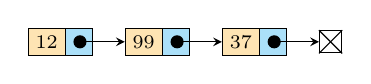
\begin{tikzpicture}[drop shadow,list/.style={rectangle split, rectangle split parts=2,
    draw, rectangle split horizontal}, >=stealth, node distance=4mm,start chain,rectangle split part fill={orangenodebg, bluenode},
]

  \node[list,on chain] (A) {12};
  \node[list,on chain] (B) {99};
  \node[list,on chain] (C) {37};
  \node[on chain,draw,inner sep=4pt] (D) {};
  \draw (D.north east) -- (D.south west);
  \draw (D.north west) -- (D.south east);
  \draw[*->] let \p1 = (A.two), \p2 = (A.center) in (\x1,\y2) -- (B);
  \draw[*->] let \p1 = (B.two), \p2 = (B.center) in (\x1,\y2) -- (C);
  \draw[*->] let \p1 = (C.two), \p2 = (C.center) in (\x1,\y2) -- (D);
\end{tikzpicture}
\end{center}
   \end{minipage}
   \begin{minipage}[c]{4.8cm}
   \begin{center}
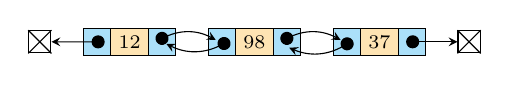
\begin{tikzpicture}[>=stealth,
        list/.style={
            rectangle split,
            rectangle split parts=3, draw,
            rectangle split horizontal, text=black,
            rectangle split part fill={bluenode, orangenodebg, bluenode}
        },
        node distance=4mm,
        start chain,
      ]

  \node[list,on chain] (A) {\nodepart{second} 12};
  \node[list,on chain] (B) {\nodepart{second} 98};
  \node[list,on chain] (C) {\nodepart{second} 37};

  \node[on chain,draw,inner sep=4pt] (D) {};
   \draw (D.north east) -- (D.south west);
  \draw (D.north west) -- (D.south east);
  \node[on chain,draw,inner sep=4pt] (E) [left= of A] {};
   \draw (E.north east) -- (E.south west);
  \draw (E.north west) -- (E.south east);

  \path[*->] let \p1 = (A.three), \p2 = (A.center) in (\x1,\y2) edge [bend left] ($(B.one)+(0,0.1)$);
  \path[*->] let \p1 = (B.three), \p2 = (B.center) in (\x1,\y2) edge [bend left] ($(C.one)+(0,0.1)$);
  \draw[*->] let \p1 = (C.three), \p2 = (C.center) in (\x1,\y2) -- (D);

  \draw[*->] ($(A.one)+(0.175,0.075)$) -- (E);
  \path[*->] ($(B.one)+(0.175,0.1)$) edge [bend left] ($(A.three)+(0.125,0.05)$);
  \path[*->] ($(C.one)+(0.15,0.1)$) edge [bend left] ($(B.three)+(0.1,0.00)$);
\end{tikzpicture}
\end{center}
\end{minipage} %\smallskip

\begin{itemize}
    \iteminfo Since there's no need to maintain contiguity, inserting/removing nodes is \bigO{1} at any position in a list, as the only adjustment you need to make is re-pointing the previous node's \code{next} pointer (and the following node's \code{prev} pointer in a doubly-linked list) instead of shifting every element. This does mean lists have \bigO{n} instead of \bigO{1} indexing, though.
    %\disadvantage Due to the lack of contiguity, lists can't use pointer arithmetic to access arbitrary indices in \bigO{1} time like arrays and vectors can, so accessing a particular index of a list takes \bigO{n} time.
    %\disadvantage Storing a sequence of numbers in a list requires more space than an array, since you have to create \code{Node} structs and pointers.
\end{itemize}

\blueheader{Linked List Operations}
% \begin{tcbraster}[raster columns=2,raster before skip=3pt, raster after skip=1pt,
%                   raster equal height, raster column skip=-.5mm]
% \begin{tcolorbox}[top=-5pt,bottom=-5pt,left=-7.5pt,right=0pt,
% %center title,toptitle=-0.6mm,
%   %bottomtitle=-0.6mm,
%   arc=0.8pt]
%               \begin{lstlisting}[style = mystyle]
% void deleteAtIndex(int idx) {
%   if (head == nullptr) { return; } // Base 1
%   else if (idx == 0) { // Base 2
%     Node* temp = head;
%     head = temp->next; delete temp;
%     return;
%   }
%   Node* ptr = head; int i = 0;
%   while (ptr && i < idx - 1) {
%     ptr = ptr->next; ++i;
%   } // if out-of-bounds, delete nothing
%   if (!ptr || !ptr->next) { return; }
%   Node* to_remove = ptr->next;
%   ptr->next = to_remove->next;
%   delete to_remove;
% }
% \end{lstlisting}
% \end{tcolorbox}
% \begin{tcolorbox}[top=-5pt,bottom=-5pt,left=-7.5pt,right=-1pt,center title,toptitle=-0.6mm,
%   bottomtitle=-0.6mm,arc=0.8pt,sharp corners,rounded corners=northeast,rounded corners=southeast]
%               \begin{lstlisting}[style = mystyle]
% void insert(int val) {
% Node* new_node = new Node{val};
% if (!head) { // if list is empty
%   head = new_node, tail = new_node;
%   return;
% }

% }
% \end{lstlisting}
% \end{tcolorbox}
% \end{tcbraster}


\titlebox{cyan!60!darkgray}{\textcolor{white}{\textbf{Recursion}}}

% Recursive functions can be separated into three categories:
% \begin{itemize}
%     \item[1.] \textbf{Linear recursive} functions make at most one recursive call to themselves for each invocation.
%     \item[2.] A \textbf{tail recursive} function is a type of linear recursive function where the recursive call is the last instruction of the function. (Note: iteration is a special case of tail recursion).
%     %invocation that makes a recursive call.
%     \item[3.] \textbf{Tree recursive} functions can make \textit{multiple} recursive calls to themselves in a single invocation.
% \end{itemize}

\begin{minipage}[c]{5.6cm}
\blueheader{Properties and Types of Recursion}

A \vocab{recursive function} is a function that is defined in terms of itself (i.e., that calls itself). Recursive functions break problems down into two types of "cases":
\begin{itemize}
    \item \textit{Base cases}, problems that can be solved without recursion (and act as the end condition for a recursive loop). Ex: $0$ and $1$ for a factorial function.
    %Ex: the base cases for a factorial function are inputs of $0$ and $1$. 
    %If a recursive function has no base cases, an infinite loop will occur, since each recursive call will always generate more calls.
    \item \textit{Recursive cases}, which the function breaks down into simpler sub-problems and then passes to itself (until the problem has been reduced to base cases).
\end{itemize} %\smallskip

%\blueheader{Memory Management Errors} \smallskip
There are three types of recursive functions:
\begin{itemize}
    \item[1.] \vocab{Linear recursive}: functions that make no more than one call to themselves for each invocation.
    \item[2.] \vocab{Tail recursive}: a type of linear recursive function whose final instruction is the recursive call.
    %invocation that makes a recursive call.
    \item[3.] \vocab{Tree recursive}: functions that can make \textit{multiple} recursive calls to themselves in one stack frame (note: they're not limited to tree data structures). 
    %functions that can make \textit{multiple} recursive calls to themselves in a single invocation (note: they're not limited to tree data structures).
\end{itemize}
   \end{minipage}
   \hspace{0pt}
\begin{minipage}[c]{4.6cm}
\begin{tcolorbox}[top=-4pt,bottom=-4pt,left=-7.5pt,right=-1pt,center title,toptitle=-0.6mm,
  bottomtitle=-0.6mm,adjusted title={\footnotesize Linear Recursion (Non-Tail)},fonttitle=\large\sffamily\bfseries]
              \begin{lstlisting}[style = mystyle]

\end{lstlisting}
   \end{tcolorbox}

   \begin{tcolorbox}[top=-4pt,bottom=-4pt,left=-7.5pt,right=-1pt,center title,toptitle=-0.6mm,
  bottomtitle=-0.6mm,adjusted title={\footnotesize Tree Recursion},fonttitle=\large\sffamily\bfseries]
              \begin{lstlisting}[style = mystyle]
bool SameTree(TreeNode* p,TreeNode* q) {
  if (!p || !q) {return (!p == !q);}
  if (p->val != q->val) {return false;}
  return SameTree(p->L, q->L) 
         && SameTree(p->R, q->R);
} // check if two trees are identical

void func(int n) {
  for (int i = 0; i < n; ++i) func(i);
} // Yes, this is tree-recursive

\end{lstlisting}
   \end{tcolorbox}
\end{minipage}

% \begin{tcbraster}[raster columns=13, raster after skip=3pt, raster before skip=3pt,
%                   raster equal height, raster column skip=-.5mm]
% \begin{tcolorbox}[top=-4pt,bottom=-4pt,left=-7.5pt,right=-1pt,center title,toptitle=-0.6mm,
%   bottomtitle=-0.6mm,boxrule=0.5pt,arc=0.8pt,raster multicolumn=4,rounded corners=northwest,rounded corners=southwest]
%               \begin{lstlisting}[style = mystyle,numbers=none]

% \end{lstlisting}
% \end{tcolorbox}
% \begin{tcolorbox}[top=-5pt,bottom=-5pt,left=-7.5pt,right=-1pt,center title,toptitle=-0.6mm,
%   bottomtitle=-0.6mm,boxrule=0.5pt,arc=0.8pt,raster multicolumn=4, sharp corners]
%               \begin{lstlisting}[style = mystyle,numbers=none]


% \end{lstlisting}
% \end{tcolorbox}
% \begin{tcolorbox}[top=-5pt,bottom=-5pt,left=-7.5pt,right=-1pt,center title,toptitle=-0.6mm,
%   bottomtitle=-0.6mm,boxrule=0.5pt,arc=0.8pt,raster multicolumn=5,sharp corners,rounded corners=northeast,rounded corners=southeast]
%               \begin{lstlisting}[style = mystyle,numbers=none]
% bool SameTree(Node* p, Node* q) {
%   if (!p || !q) { 
%     return (!p == !q); 
%   }
%   if (p->val != q->val) { 
%     return false; 
%   }
%   return SameTree(p->L, q->L) 
%       && SameTree(p->R, q->R);
% }
% \end{lstlisting}
% \end{tcolorbox}
% \end{tcbraster} \smallskip

\begin{itemize}
    \itemwarning A recursive call being on the last line of a function does NOT guarantee that the function is tail recursive—the recursive call must be the last \textit{instruction} executed by the function.
\end{itemize}

 \begin{tcolorbox}[top=-4pt,bottom=-4pt,left=-7.5pt,right=-1pt,center title,toptitle=-0.6mm,
  bottomtitle=-0.6mm,before skip = 3pt, after skip = 3pt,
  %adjusted title={\footnotesize Ways to Create and Use a C-String},fonttitle=\large\sffamily\bfseries
  ]
              \begin{lstlisting}[style = mystyle]
int factorial(int n) {
  return (n <= 1) ? 1 : n * factorial(n - 1);
} /* This is NOT tail-recursive because the last instruction the function executes is 
     multiplying the recursive result by n, not the recursive call itself. */
\end{lstlisting}
\end{tcolorbox}



% A \textbf{linear recursive} function makes at most one recursive call to itself each time it's invoked.

\blueheader{Memory Usage of Recursive Functions}

\textit{Non-tail} linear recursive functions allocate an additional stack frame with each recursive call. However, the compiler can optimize a tail recursive function to reuse the same stack frame, which means that tail-recursive functions can be optimized to use a constant number of stack frames.

\begin{itemize}
    \itemwarning The total number of recursive calls a function makes to itself does not indicate its space complexity, since not all stack frames have to exist at the same time. Instead, look at the \underline{number of return statements until the base case}. For example, a recursive algorithm to traverse a balanced BST of height $h$ uses a maximum of \bigO{h} space—not \bigO{2^h} space—at any given time.
\end{itemize}

% A \textbf{tail recursive} function is a type of linear recursive function where the recursive call is the last thing that happens in every invocation that makes a recursive call.

% A function is \textbf{tree recursive} if it can make \textit{multiple} recursive calls to itself in a single invocation.

\blueheader{Structural Recursion}

\vocab{Structural recursion} is when an abstract data type is defined in terms of itself. The \code{Node} structs of a linked list are one example: each \code{Node} contains a pointer to another \code{Node}. Recursive structures have base cases and recursive cases just like recursive functions do: for a linked list, the "base case" is an empty list, and the recursive cases are non-empty lists.

% \begin{itemize}
%     \iteminfo Problems involving recursive structures lend themselves well to recursive solutions.
% \end{itemize}

\blueheader{Recursion vs Iteration (and Converting Between Them)}

\titlebox{blue!45!gray!90!lightgray}{Binary Search Trees and Maps}

   \begin{minipage}[c]{7.3cm} 
   \blueheader{Binary Search Trees}
   
   A \textit{binary tree} is a tree data structure where each \textit{node} points to at most 2 children. A \vocab{binary \textit{search} tree} is a binary tree where, for \textit{any} node, every node in the left subtree has a lower value and every node in the right subtree has a greater value. (An empty tree is also a BST.) \smallskip
   %each node in the left subtree has a strictly lower value than the \textit{root}, and each node in the right subtree has a strictly greater value than the root (this property applies recursively—every subtree of a BST is itself a BST). \smallskip

    A BST is \vocab{balanced} if the heights of the left and right subtrees at any node differ by no more than $1$, so the height of a balanced BST with $n$ nodes is roughly $\log_2{(n)}$. A \vocab{leaf} of a BST is a childless node.
    \smallskip
   
% \begin{itemize}
%     \iteminfo If a node has only one child, whether you view the child node as the "left" or "right" node will depend on its value.
% \end{itemize} \smallskip

    \blueheader{BST Traversal}
    
   There are multiple ways to traverse a binary tree:
   \begin{itemize}
       \item[1.] \vocab{Inorder traversal}: recursively process the \textit{left} subtree $\rightarrow$ process the \textit{head} (current) node $\rightarrow$ recursively process the \textit{right} subtree. %(For a binary \textit{search} tree, this visits nodes in ascending order of value.)
       \item[2.] \vocab{Preorder traversal}: process the \textit{head} (current) node $\rightarrow$ recursively process the \textit{left} subtree $\rightarrow$ recursively process the \textit{right} subtree.
       \item[3.] \vocab{Postorder traversal}: recursively process the \textit{left} subtree $\rightarrow$ recursively process the \textit{right} subtree. $\rightarrow$ process the \textit{head}.
       %recursively visit all of the nodes of one subtree before moving to the other subtree.
   \end{itemize}

    \begin{itemize}
        \iteminfo Inorder traversal of a BST visits nodes by ascending value. 
    \end{itemize}
    
    %Use preorder traversal to visit them in left-right order. Both methods are \bigO{n} since you'll visit every node in the tree.
   
   %\textbf{in-order traversal}, which involves visiting nodes in ascending order of their values, and \textbf{pre-order traversal}
      %A binary tree is a tree data structure where each \textit{node} has $\leq$ 2 children. A \textbf{BST} is a binary tree that has a \textit{root} with two subtrees such that the value of each node in the left subtree is strictly less than that of the root node, and the value of each node in the right subtree is strictly greater than that of the root node (and the two subtrees are themselves BSTs). An empty tree also counts as a BST.
    \end{minipage}
    \hspace{0pt}
    \begin{minipage}[c]{2.9cm}
    \begin{center}
        
    %\begin{figure}[H]
\begin{forest}
for tree={
blur shadow={ shadow scale=1, shadow xshift=.1ex, shadow yshift=-.15ex,
  opacity=.2, fill=black, every shadow,},
    grow=south,
    circle, draw, minimum size=3.5ex, inner sep=1pt,
    opacity=1,
    s sep=3mm,edge={->,>=stealth},
}
[\textbf{51},fill=Green!15,draw = Green!75!black,semithick
    [5,fill=orangenodebg,draw = orangenodeborder,semithick,semithick
        [1,fill=orangenodebg,draw = orangenodeborder,semithick,semithick]
        [43,fill=bluenode!50,draw = bluenodeborder!90!black,semithick
            [8,fill=orangenodebg,draw = orangenodeborder,semithick,semithick]
        ]
    ]
    [87,fill=bluenode!50,draw = bluenodeborder!90!black,semithick
        [52,fill=orangenodebg,draw = orangenodeborder,semithick,semithick
            [83,fill=bluenode!50,draw = bluenodeborder!90!black,semithick]
        ]
    ]
]
\end{forest}
\vspace{3pt}
    %\end{figure}

    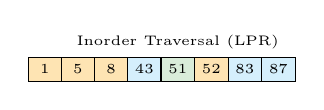
\begin{tikzpicture}[rect/.style={draw,thin,minimum width=1.5em,
    minimum height=1.1em,alias=tmp,fill=bluenode!50},>={Stealth}]
 % \path[nodes=rect] node(r0){\footnotesize6} node[above right=-1.40em and 0.75em of tmp](r1){{\footnotesize5}}
 \path[nodes=rect] 
node[fill=orangenodebg](r0){\footnotesize1} 
node[fill=orangenodebg,right=-\pgflinewidth of tmp](r1){{\footnotesize5}}
node[fill=orangenodebg,right=-\pgflinewidth of tmp](r2){{\footnotesize8}}
node[right=-\pgflinewidth of tmp](r3){{\footnotesize43}}
node[fill=Green!15,right=-\pgflinewidth of tmp](r4){{\footnotesize51}}
node[fill=orangenodebg,right=-\pgflinewidth of tmp](r5){{\footnotesize52}}
node[right=-\pgflinewidth of tmp](r6){{\footnotesize83}}
node[right=-\pgflinewidth of tmp](r6){{\footnotesize87}};
 %node[above right=-0.0em and 0.35em of tmp](r6){{\footnotesize6}}
% foreach \i in {1,...,6} {node[right=-\pgflinewidth of tmp](r\i){\footnotesize\i}};
 %node[above right=-0.0em and 0.35em of tmp](r6){{\footnotesize6}};
 \path[nodes={}] 
    (r1.north west) node[above right]{}
    (r4.north) node[above]{\footnotesize Inorder Traversal (LPR)}
    (r4.north east) node[above left]{};
 %\draw[red!60!gray,-{>[scale=0.75]}](r1.west)--++(-0:-0.20mm) to[out=0,in=0] node[above left]{} (r0.east);
 %\draw[blue!60!lightgray,-{>[scale=0.75]}](r6.south) to[out=-90,in=0] node[above right]{} (r5.east);
%\draw [{<[scale=0.75]}-, black] (r1.south)--++(-90:2.5mm) node[below,yshift=0.75mm] {\lstinline[basicstyle=\tiny]{front}};
\end{tikzpicture} 

\vspace{3pt}
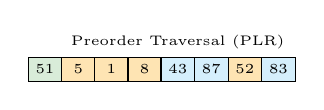
\begin{tikzpicture}[rect/.style={draw,thin,minimum width=1.5em,
    minimum height=1.1em,alias=tmp,fill=bluenode!50},>={Stealth}]
 % \path[nodes=rect] node(r0){\footnotesize6} node[above right=-1.40em and 0.75em of tmp](r1){{\footnotesize5}}
 \path[nodes=rect] 
node[fill=Green!15](r0){\footnotesize51} 
node[fill=orangenodebg,right=-\pgflinewidth of tmp](r1){{\footnotesize5}}
node[fill=orangenodebg,right=-\pgflinewidth of tmp](r2){{\footnotesize1}}
node[fill=orangenodebg,right=-\pgflinewidth of tmp](r3){{\footnotesize8}}
node[fill=bluenode!50,right=-\pgflinewidth of tmp](r4){{\footnotesize43}}
node[fill=bluenode!50,right=-\pgflinewidth of tmp](r5){{\footnotesize87}}
node[fill=orangenodebg,right=-\pgflinewidth of tmp](r6){{\footnotesize52}}
node[right=-\pgflinewidth of tmp](r6){{\footnotesize83}};
 %node[above right=-0.0em and 0.35em of tmp](r6){{\footnotesize6}}
% foreach \i in {1,...,6} {node[right=-\pgflinewidth of tmp](r\i){\footnotesize\i}};
 %node[above right=-0.0em and 0.35em of tmp](r6){{\footnotesize6}};
 \path[nodes={}] 
    (r1.north west) node[above right]{}
    (r4.north) node[above]{\footnotesize Preorder Traversal (PLR)}
    (r4.north east) node[above left]{};
 %\draw[red!60!gray,-{>[scale=0.75]}](r1.west)--++(-0:-0.20mm) to[out=0,in=0] node[above left]{} (r0.east);
 %\draw[blue!60!lightgray,-{>[scale=0.75]}](r6.south) to[out=-90,in=0] node[above right]{} (r5.east);
%\draw [{<[scale=0.75]}-, black] (r1.south)--++(-90:2.5mm) node[below,yshift=0.75mm] {\lstinline[basicstyle=\tiny]{front}};
\end{tikzpicture}

\vspace{3pt}
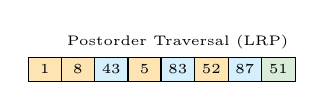
\begin{tikzpicture}[rect/.style={draw,thin,minimum width=1.5em,
    minimum height=1.1em,alias=tmp,fill=bluenode!50},>={Stealth}]
 % \path[nodes=rect] node(r0){\footnotesize6} node[above right=-1.40em and 0.75em of tmp](r1){{\footnotesize5}}
 \path[nodes=rect] 
node[fill=orangenodebg](r0){\footnotesize1} 
node[fill=orangenodebg,right=-\pgflinewidth of tmp](r1){{\footnotesize8}}
node[fill=bluenode!50,right=-\pgflinewidth of tmp](r2){{\footnotesize43}}
node[fill=orangenodebg,right=-\pgflinewidth of tmp](r3){{\footnotesize5}}
node[fill=bluenode!50,right=-\pgflinewidth of tmp](r4){{\footnotesize83}}
node[fill=orangenodebg,right=-\pgflinewidth of tmp](r5){{\footnotesize52}}
node[fill=bluenode!50,right=-\pgflinewidth of tmp](r6){{\footnotesize87}}
node[fill=Green!15,right=-\pgflinewidth of tmp](r6){{\footnotesize51}};
 %node[above right=-0.0em and 0.35em of tmp](r6){{\footnotesize6}}
% foreach \i in {1,...,6} {node[right=-\pgflinewidth of tmp](r\i){\footnotesize\i}};
 %node[above right=-0.0em and 0.35em of tmp](r6){{\footnotesize6}};
 \path[nodes={}] 
    (r1.north west) node[above right]{}
    (r4.north) node[above]{\footnotesize Postorder Traversal (LRP)}
    (r4.north east) node[above left]{};
 %\draw[red!60!gray,-{>[scale=0.75]}](r1.west)--++(-0:-0.20mm) to[out=0,in=0] node[above left]{} (r0.east);
 %\draw[blue!60!lightgray,-{>[scale=0.75]}](r6.south) to[out=-90,in=0] node[above right]{} (r5.east);
%\draw [{<[scale=0.75]}-, black] (r1.south)--++(-90:2.5mm) node[below,yshift=0.75mm] {\lstinline[basicstyle=\tiny]{front}};
\end{tikzpicture}
    \end{center}
    \end{minipage}

\begin{tcbraster}[raster columns=12, raster after skip=3pt, raster before skip=3pt,
                  raster equal height, raster column skip=-.5mm]
\begin{tcolorbox}[top=-5pt,bottom=-5pt,left=-7.5pt,right=-1pt,center title,toptitle=-0.6mm,
  bottomtitle=-0.6mm,boxrule=0.5pt,arc=0.8pt,raster multicolumn=4,rounded corners=northwest,rounded corners=southwest]
{\lstset{
escapeinside=@@,
literate=% Colors the digits
   *{0}{{{\color{vscode_green!100!black}0}}}1
    {1}{{{\color{vscode_green!100!black}1}}}1
    {2}{{{\color{vscode_green!100!black}2}}}1
    {3}{{{\color{vscode_green!100!black}3}}}1
    {4}{{{\color{vscode_green!100!black}4}}}1
    {5}{{{\color{vscode_green!100!black}5}}}1
    {6}{{{\color{vscode_green!100!black}6}}}1
    {7}{{{\color{vscode_green!100!black}7}}}1
    {8}{{{\color{vscode_green!100!black}8}}}1
    {9}{{{\color{vscode_green!100!black}9}}}1
%{<<}{{{\color{operator}<\/<}}}2
}
              \begin{lstlisting}[style = mystyle,numbers=none]
void preOrder(Node* p) {
  if (!p) return;
  process(p->val);
  preOrder(p->left);
  preOrder(p->right);
} // preorder traversal
\end{lstlisting}
}
\end{tcolorbox}
\begin{tcolorbox}[top=-5pt,bottom=-5pt,left=-7.5pt,right=-1pt,center title,toptitle=-0.6mm,
  bottomtitle=-0.6mm,boxrule=0.5pt,arc=0.8pt,raster multicolumn=4, sharp corners]
{\lstset{
escapeinside=@@,
literate=% Colors the digits
   *{0}{{{\color{vscode_green!100!black}0}}}1
    {1}{{{\color{vscode_green!100!black}1}}}1
    {2}{{{\color{vscode_green!100!black}2}}}1
    {3}{{{\color{vscode_green!100!black}3}}}1
    {4}{{{\color{vscode_green!100!black}4}}}1
    {5}{{{\color{vscode_green!100!black}5}}}1
    {6}{{{\color{vscode_green!100!black}6}}}1
    {7}{{{\color{vscode_green!100!black}7}}}1
    {8}{{{\color{vscode_green!100!black}8}}}1
    {9}{{{\color{vscode_green!100!black}9}}}1
%{<<}{{{\color{operator}<\/<}}}2
}
              \begin{lstlisting}[style = mystyle,numbers=none]
void inOrder(Node* p) {
  if (!p) return;
  inOrder(p->left);
  process(p->val);
  inOrder(p->right);
} // inorder traversal
\end{lstlisting}
}
\end{tcolorbox}
\begin{tcolorbox}[top=-5pt,bottom=-5pt,left=-7.5pt,right=-1pt,center title,toptitle=-0.6mm,
  bottomtitle=-0.6mm,boxrule=0.5pt,arc=0.8pt,raster multicolumn=4,sharp corners,rounded corners=northeast,rounded corners=southeast]
{\lstset{
escapeinside=@@,
literate=% Colors the digits
   *{0}{{{\color{vscode_green!100!black}0}}}1
    {1}{{{\color{vscode_green!100!black}1}}}1
    {2}{{{\color{vscode_green!100!black}2}}}1
    {3}{{{\color{vscode_green!100!black}3}}}1
    {4}{{{\color{vscode_green!100!black}4}}}1
    {5}{{{\color{vscode_green!100!black}5}}}1
    {6}{{{\color{vscode_green!100!black}6}}}1
    {7}{{{\color{vscode_green!100!black}7}}}1
    {8}{{{\color{vscode_green!100!black}8}}}1
    {9}{{{\color{vscode_green!100!black}9}}}1
%{<<}{{{\color{operator}<\/<}}}2
}
              \begin{lstlisting}[style = mystyle,numbers=none]
void postOrder(Node* p) {
  if (!p) return;
  postOrder(p->left);
  postOrder(p->right);
  process(p->val);
} // postorder traversal
\end{lstlisting}
}
\end{tcolorbox}
\end{tcbraster}

%\vspace*{-\baselineskip} 

\blueheader{Recursive Big Three}

\smallskip
\textcolor{headcolor}{\textbf{Operations on BSTs vs Sorted/Unsorted Sets}}

\textbf{Search}: due to the sorting invariant, searching a balanced BST for a value takes \bigO{\log n} time.

\begin{tcolorbox}[top=-5pt,bottom=-5pt,left=-7.5pt,right=-0pt,middle=-5pt,
   before skip = 3pt,
 center title,toptitle=-0.6mm,middle=-5pt,
 bottomtitle=-0.6mm,
  adjusted title={Recursive Binary Search},fonttitle=\sffamily\bfseries
  ]
\begin{lstlisting}[style = mystyle]
template <typename Iter, typename T>
int @\textcolor{clr-function}{binarySearch}@(Iter left, Iter right, const T& val) {
@\indentrule@int size = (right - left);
@\indentrule@if (size <= 0) return -1;
@\indentrule@Iter mid = left + (size / 2);
@\indentrule@if (*mid == val) return (mid - left);
@\indentrule@if (*mid > val) return binarySearch(left, mid, val);
@\indentrule@return binarySearch(mid + 1, right, val);
} // eliminates half the search space each loop
\end{lstlisting}
\end{tcolorbox}


\begin{itemize}
    \iteminfo \code{std::map} and \code{std::set} are implemented using \textit{self-balancing} binary search trees, which is how they maintain $\bigTheta(\log n)$ insertion, removal, and searching even in the worst case.
\end{itemize}

% \def\arraystretch{1.15}
% \begin{table}[htbp]
% \begin{NiceTabular*}{\textwidth}{|c|c|c|c|c|c|c|c|c|c|}[color-inside,corners=NW]
% \CodeBefore
% \rowcolor{gray!50}{1}
% \rowcolors{2}{evenrow}{white}
% \Body
% \hhline{~----}
% &  \rowcolor{graycell} \Block{1-2}{\bfseries{Array-Based Set}} & & \Block{1-2}{\bfseries{Sorted Array-Based Set}} & & \Block{1-2}{\bfseries{Balanced BST}} & & \Block{1-2}{\textbf{Linked List}} & & \\
% \hhline{~----}
% & Average & Worst & Average & Worst & Average & Worst & Average & Worst & \\
% \hhline{-----}
% \cellcolor{graycell} Insert & \bigO{n} & \bigO{n} & \bigO{n} & \bigO{\log n}  & \bigO{1} & \bigO{1} \\
% \hhline{-----}
% \cellcolor{graycell} Erase & \bigO{n} & \bigO{n} & \bigO{n} & \bigO{\log n} & \bigO{1} & \bigO{1} \\
% \hhline{-----}
% \cellcolor{graycell} Find & \bigO{n} & \bigO{n} & \bigO{\log n} & \bigO{\log n} & \bigO{n} & \bigO{n} \\
% \hhline{-----}
% \end{NiceTabular*}
% \end{table}



% \vspace*{-\baselineskip}
% \begin{center}
% \setlength\cellspacetoplimit{1.5pt}
% \setlength\cellspacebottomlimit{1.5pt}
% \resizebox{\linewidth}{!}{\begin{tabular}{|Sc|Sc|Sc|Sc|Sc|Sc|Sc|Sc|Sc|Sc|}
% %\hline
% % \hhline{~|-|-|-|-|-|-|-|-|-|}
% %  \multicolumn{1}{p{0.5cm}|}{} & \multicolumn{9}{|Sc|}{{\textbf{Time complexities of insert/remove/search on data structures (worst, best, average)}} \cellcolor{gray!12}} \\
%  \hhline{~|-|-|-|-|-|-|-|-|-|}
% \multicolumn{1}{p{0.5cm}|}{} & \multicolumn{3}{Sc|}{Unsorted Set \cellcolor{gray!12}} & \multicolumn{3}{Sc|}{Sorted Set \cellcolor{gray!12}} & \multicolumn{3}{Sc|}{Binary Search Tree* \cellcolor{gray!12}} \\ 
% \hhline{~|-|-|-|-|-|-|-|-|-|}
% \multicolumn{1}{p{0.5cm}|}{} & \cellcolor{gray!12} Worst & \cellcolor{gray!12} Best & \cellcolor{gray!12} Average & \cellcolor{gray!12} Worst & \cellcolor{gray!12} Best & \cellcolor{gray!12} Average & \cellcolor{gray!12} Worst & \cellcolor{gray!12} Best & \cellcolor{gray!12} Average \\ 
% \hline 
% \myinline{insert} \cellcolor{gray!12} & $\mathrm{O}(n)$ & $\mathrm{\Omega}(n)$ & $\mathrm{\Theta}(1)$ & $\mathrm{O}(n)$ & $\mathrm{\Omega}(n)$ & $\mathrm{\Theta}(n)$ & $\mathrm{O}(n)$ & $\mathrm{\Omega}(n)$ & $\mathrm{\Theta}(\log n)$ \\ 
% \hline
% \myinline{remove} \cellcolor{gray!12} & $\mathrm{O}(n)$ & $\mathrm{\Omega}(n)$ & $\mathrm{\Theta}(1)$ & $\mathrm{O}(n)$ & $\mathrm{\Omega}(n)$ & $\mathrm{\Theta}(n)$ & $\mathrm{O}(n)$ & $\mathrm{\Omega}(n)$ & $\mathrm{\Theta}(\log n)$ \\ 
% \hline
% \myinline{contains} \cellcolor{gray!12} & $\mathrm{O}(n)$ & $\mathrm{\Omega}(n)$ & $\mathrm{\Theta}(1)$ & $\mathrm{O}(n)$ & $\mathrm{\Omega}(n)$ & $\mathrm{\Theta}(n)$ & $\mathrm{O}(n)$ & $\mathrm{\Omega}(1)$ & $\mathrm{\Theta}(\log n)$ \\ 
% %\hline 
% %{\lstinline |size, constructor|} & $\mathrm{O}(1)$ \cellcolor{green!15} & $\mathrm{O}(1)$ \cellcolor{green!15} & $\mathrm{O}(1)$ \cellcolor{green!15} &  $\mathrm{O}(1)$ \cellcolor{green!15} & $\mathrm{O}(1)$ \cellcolor{green!15} \\ 
% \hline 
% %{\lstinline |access|} & $\mathrm{O}(1)$ \cellcolor{green!15} & $\mathrm{O}(1)$ \cellcolor{green!15} & $\mathrm{O}(n)$ \cellcolor{yellow!22} &  $\mathrm{O}(n)$ \cellcolor{yellow!22} &  $\mathrm{O}(1)$ \cellcolor{green!15} \\ 
% %\hline 
% \end{tabular}}

{\footnotesize *Where $n$ = number of nodes in the tree}
%\end{center}
%\vspace*{-\baselineskip} 

Best case: $\Omega(n)$

Worst case: $\mathrm{O}(n)$

Average case: $\Theta(n)$

\titlebox{green!50!black}{Iterators and Functors}

\vocab{Functors (function objects)}: \textit{first-class} entities that provide the same interface as a function. They can be created from classes that overload the function-call operator, i.e., \code{operator()}.
\begin{itemize}
    \iteminfo First-class entities can \textit{store state} (store and access information), be created at runtime, and be passed as an argument to/returned by a function.
    \iteminfo \code{operator()} can only be overloaded from within a class body. It and \code{operator[]} are also the only operators that can be overloaded as \code{static} member functions.
\end{itemize}

\vocab{Function Pointers}

\vocab{Iterators} are a type of object that are designed to emulate the interface of a pointer.

{
\setlength{\tabcolsep}{0.75em}
\setlength\cellspacetoplimit{1.5pt}
\setlength\cellspacebottomlimit{1.5pt}
\resizebox{\linewidth}{!}
{\begin{tabular}{|Sc|Sc|Sc|Sc|Sc|Sc|Sc|Sc|Sc|Sc|}
%\hline
 %\multicolumn{6}{|Sc|}{{\textbf{Time Complexities of Operations on Containers of Size $n$ }} \cellcolor{gray!15}} \\
\hhline{~|-|-|-|-|-|-|-|-|-|}
\multicolumn{1}{Sc|}{} & \myinline{std::sort(it1,it2)} \cellcolor{gray!15} & \myinline{it2 - it1} \cellcolor{gray!15} & \myinline{it[n]} \cellcolor{gray!15} & \myinline{it += n} \cellcolor{gray!15} & \myinline{it1 < it2} \cellcolor{gray!15} & \myinline{--it} \cellcolor{gray!15} & \myinline{++it} \cellcolor{gray!15} & \myinline{it1 == it2} \cellcolor{gray!15} & \myinline{*it} \cellcolor{gray!15} \\
\hline
Random Access \cellcolor{gray!15} & \textcolor{true-green}{\faCheck} Yes & \textcolor{true-green}{\faCheck} Yes & \textcolor{true-green}{\faCheck} Yes & \textcolor{true-green}{\faCheck} Yes & \textcolor{true-green}{\faCheck} Yes & \textcolor{true-green}{\faCheck} Yes & \textcolor{true-green}{\faCheck} Yes & \textcolor{true-green}{\faCheck} Yes & \textcolor{true-green}{\faCheck} Yes \\
\hline
\rowcolor{evenrow} Bidirectional \cellcolor{gray!15} & \textcolor{false-red}{\faTimes} No & \textcolor{false-red}{\faTimes} No & \textcolor{false-red}{\faTimes} No & \textcolor{false-red}{\faTimes} No & \textcolor{false-red}{\faTimes} No & \textcolor{true-green}{\faCheck} Yes & \textcolor{true-green}{\faCheck} Yes & \textcolor{true-green}{\faCheck} Yes & \textcolor{true-green}{\faCheck} Yes \\
\hline
Forward \cellcolor{gray!15} & \textcolor{false-red}{\faTimes} No & \textcolor{false-red}{\faTimes} No & \textcolor{false-red}{\faTimes} No & \textcolor{false-red}{\faTimes} No & \textcolor{false-red}{\faTimes} No & \textcolor{false-red}{\faTimes} No & \textcolor{true-green}{\faCheck} Yes &  \textcolor{true-green}{\faCheck} Yes &  \textcolor{true-green}{\faCheck} Yes \\
\hline
\end{tabular}}
}

{\setlength{\tabcolsep}{0.5em}
\resizebox{\linewidth}{!}{\begin{tabular}{|Sc|Sc|Sc|Sc|Sc|Sc|}
% \hline
%\multicolumn{6}{|Sc|}{{\textbf{Time Complexities of Operations on Containers of Size $n$ }} \cellcolor{gray!15}} \\
\hline 
Iterator \cellcolor{gray!15} & \myinline{array<T,N>::iterator} \cellcolor{gray!15} & \myinline{vector<T>::iterator} \cellcolor{gray!15} & \myinline{list<T>::iterator} \cellcolor{gray!15} & \myinline{map<Key,T>::iterator} \cellcolor{gray!15} & \myinline{set<Key>::iterator} \cellcolor{gray!15}  \\ 
\hline 
Iterator Class \cellcolor{gray!15} & Random Access & Random Access & Bidirectional & Bidirectional & Bidirectional\\ 
\hline
Container Resizing \cellcolor{gray!15} & N/A &  \makecell{All iterators invalidated} & Dynamic & Empty container &  Linked \\ 
\hline
Insertion \cellcolor{gray!15} & Sequential &  \makecell{Iterators at/above point of \\ insertion are invalididated} & Unaffected & Unaffected &  Unaffected \\ 
\hline 
Erasure \cellcolor{gray!15} & Sequential &  \makecell{Iterators at/above point of \\ erasure are invalididated} & Dynamic & Empty container &  Linked \\ 
\hline 
\end{tabular}}}

\smallskip
\blueheader{Friend Classes}

Declaring a class \code{S} as a \code{friend} of class \code{T} makes the private data members of \code{S} accessible in the scope of \code{T} (but not vice versa—\code{T}'s private members don't become accessible to \code{S}).

 \begin{tcolorbox}[top=-4pt,bottom=-4pt,left=-7.5pt,right=-1pt,center title,toptitle=-0.6mm,
  bottomtitle=-0.6mm,before skip = 3pt, after skip = 3pt,
  %adjusted title={\footnotesize Ways to Create and Use a C-String},fonttitle=\large\sffamily\bfseries
  ]
\begin{lstlisting}[style = mystyle]
friend class F;
friend F;
\end{lstlisting}
\end{tcolorbox}


\titlebox{violet!80!Lavender}{Error Handling and Exceptions}

\begin{itemize}
    \iteminfo A \code{try} block can have multiple \code{catch} blocks associated with it.
\end{itemize}

Uncaught exceptions will make the program terminate.

\titlebox{violet!80!Lavender}{C++ Stuff and Impostor Syndrome}

%Imposter syndrome characteristics: 1) attribute success to external factors; 2) fear
%being revealed as a fraud; 3) convinced not good enough; 4) hard to accepting
%compliments for accomplishments.

\vocab{Impostor syndrome} is characterized by doubt in one's abilities  that aren't backed up by evidence and an inability to recognize/take credit for one's achievements. These feelings are common and can affect anyone (although people from underrepresented groups may be more susceptible to it).

A \vocab{static member function} does \textit{not} have access to the \code{this} pointer and also can't access non-\code{static} data members (reminder: \code{static} members are "shared" between all instances of a class).

Templates and function overloading are forms of \vocab{compile-time polymorphism}, while subtype polymorphism is a form of \vocab{runtime polymorphism}.

\textcolor{headcolor}{\textbf{Container ADTs}} 

\textbf{\code{static}} \textbf{keyword}: used to make one copy of a class data member "shared" between all instances of that class. A \code{static} data member has static storage duration but exists only within the scope of a class. 



\begin{minipage}[h]{4.0cm}
   \textbf{stack}: a container that's designed to operate in a LIFO order.

   \textbf{queue}: a container designed to operate in a first-in/first-out (FIFO) order.
    \end{minipage}
    \hspace{0pt}
   \begin{minipage}[h]{6.2cm} 
       \setlength\cellspacetoplimit{1.5pt}
\setlength\cellspacebottomlimit{1.5pt}
{\setlength{\tabcolsep}{0.6em}
\resizebox{\linewidth}{!}{\begin{tabular}{*{7}{|Sc}|}
    {\graycell Container} & \multicolumn{6}{Sc|}{\footnotesize Interface Operations - Optimal Implementations are All $\mathrm{O}(1)$ \graycell} \\
    \hline
   Stack  \graycell & \myinline{empty} & \myinline{size} & \multicolumn{2}{Sc|}{\myinline{top (next to pop)}} & \myinline{push_back} & \myinline{pop_back} \\
    \hline
    Queue \graycell & \myinline{empty} & \myinline{size} & \myinline{front (next)} & \myinline{back (last)} & \myinline{push_back} & \myinline{pop_front} \\
  \hline
\end{tabular}}} \\
    \end{minipage}
    
\begin{itemize}

\iteminfo An efficient way to implement a queue is to create a vector with free space at both ends (a \textbf{ring/circular buffer}). This requires keeping track of the data's "head" (inclusive) and "tail" (exclusive).
\end{itemize}

\begin{minipage}[h]{5.2cm}
\setlength\cellspacetoplimit{1pt}
\setlength\cellspacebottomlimit{1pt}
{\setlength{\tabcolsep}{0.6em}
\resizebox{\linewidth}{!}{\begin{tabular}{*{6}{|Sc}|}
    \hline
   \multicolumn{5}{|Sc|}{\footnotesize Useful \myinline{std::vector} Functions and Constructors \graycell}  \\
    \hline
    {\lstinline|.size()|} & {\lstinline|v[i]/.at(i)|} & {\lstinline|.push_back(val)|} & {\lstinline|.pop_back()|} & {\lstinline|.resize(n)|} \\
    \hline
    {\lstinline|.front()|} & {\lstinline|.back()|} & {\lstinline|.erase(iterator)|} & {\lstinline|.empty()|} & {\lstinline|.clear()|} \\
    \hline
    \multicolumn{3}{|Sc|}{\footnotesize{\lstinline|vector<T> v2(v1.begin(), v1.end())|}} & \multicolumn{2}{Sc|}{\footnotesize {\lstinline|vector<T> v2(v1)|}} \\
  \hline
\end{tabular}}} 

\end{minipage}
\hspace{0pt}
\begin{minipage}[h]{5.0cm} \smallskip

{\setlength{\tabcolsep}{0.6em}
\resizebox{\linewidth}{!}{\begin{tabular}{|Sc|Sc|Sc|Sc|Sc|Sc|Sc|Sc|}

% \hline 
% Operation \graycell & Unsorted Set\textcolor{red}{*} \graycell & Sorted Set\textcolor{red}{*} \graycell & Stack \graycell & Queue \graycell & Array \graycell & List \graycell \\ 
% \hline 
% {\lstinline |insert/remove|} \graycell & $\mathrm{O}(n)$ & $\mathrm{O}(n)$ & $\mathrm{O}(1)$ & $\mathrm{O}(1)$  & $\mathrm{O}(n)$ & $\mathrm{O}(1)$ \\ 
% \hline
% {\lstinline |search| } \graycell &  $\mathrm{O}(n)$ & $\mathrm{O}(\log n)$ & $\mathrm{O}(n)$ & $\mathrm{O}(n)$ & $\mathrm{O}(n)$ & $\mathrm{O}(n)$ \\ 
% \hline 
% {\lstinline |access|} \graycell & $\mathrm{O}(1)$ & $\mathrm{O}(1)$ & $\mathrm{O}(n)$ &  $\mathrm{O}(n)$ &  $\mathrm{O}(1)$ & $\mathrm{O}(n)$ \\ 
% \hline 

\end{tabular}
}
}
{\scriptsize{\textcolor{red}{*} These refer to the array-based sets we saw in class, \textit{not} STL sets.}}

\end{minipage}%

\smallskip
\textcolor{headcolor}{\textbf{\Cpp Standard Library Containers}} 

\codedef{std::array}: Containers with \textit{compile-time constant} sizes that store elements in contiguous memory. 
%Note that size is part of the template parameter for a \code{std::array}.

\codedef{std::vector}: resizable containers that store elements at the front and free space at the back.

\begin{itemize}

\itemwarning Element insertions/deletions will invalidate \code{std::vector} iterators \textit{at and after} the modified index. Also, any operation that changes the maximum capacity of a vector invalidates all existing iterators.
\end{itemize}

\textbf{\code{std::list}}: a container whose elements are linked via pointers (i.e., in non-contiguous memory).

\textbf{\code{std::map}}: an associative array that maps unique keys to values. Keys act like indexes for a map.

\textbf{\code{std::set}}: an associative sorted container that only stores unique keys.
\begin{itemize}

\iteminfo Removing an element from a \code{std::list}, \code{std::set}, or \code{std::map} only invalidates iterators to the removed element. Also, inserting an element doesn't ever invalidate iterators for those containers.
\end{itemize}

\smallskip
\begin{minipage}[c]{5.1cm} 
   \begin{tcolorbox}[,toptitle=-0.6mm,
bottomtitle=-0.6mm,top=-4pt,bottom=-4pt,middle=-5pt,left=-7.5pt,right=0pt,,
adjusted title={ \Cpp Standard Library Containers},fonttitle=\sffamily\bfseries
   %segmentation style={solid}
   ]
              {\lstset{literate=
    *{const}{{{\color{blue} \textbf{const}}}}5
    %{<<}{{{\color{operator}<\/<}}}2
}
\begin{lstlisting}[style = mystyle]
std::array<int, 4> arr = {-4,0,3,6};
std::array @arr2@{1, 2}; // Only way to omit size
std::list<int> doubly_linked = {1,2,3};
std::forward_list<int> singly_linked = {4,5,6};
std::set<int> nums = {3,2,2,1}; // {1,2,3}

std::map<string, int> EECS = { {"Bill", 183} };
cout << EECS["Bill"] << endl; // prints 183
// Two ways to insert into a map:
EECS["Emily"] = 203;
EECS.insert(pair<string, int>("James", 280));
\end{lstlisting}
}
\end{tcolorbox} 
   \end{minipage}
   \hspace{0pt}
   \begin{minipage}[c]{5.1cm}
   \begin{tcolorbox}[,toptitle=-0.6mm,
bottomtitle=-0.6mm,top=-4pt,bottom=-4pt,middle=-5pt,left=-7.5pt,right=-0pt,,
adjusted title={ Useful \myinlinewhite{std::map} functions},fonttitle=\sffamily\bfseries
   %segmentation style={solid}
   ]
              {
    \lstset{
    escapeinside=@@,
    literate=
    %{const}{{{\color{blue} \textbf{const}}}}5
    %{<<}{{{\color{operator}<\/<}}}2
}
\begin{lstlisting}[style = mystyle,numbers=none]
// Returns iterator to the pair with Key == k
// Returns .end() iterator if no such pair exists
iterator find(const @\color{clr-type}{Key\_type}@& k) const;

// Inserts a <key, value> std::pair into a map
// Returns <iterator, false> if Key already in use
pair<iterator,bool> insert(const @\color{clr-type}{Pair\_type}@& @pair@);

/* Finds or enters a value for a given key, then 
returns a reference to the associated value */
@\color{clr-type}{Value\_type}@& operator[](const @\color{clr-type}{Key\_type}@& key);
\end{lstlisting}
}
\end{tcolorbox} 

\end{minipage}

\smallskip

% {\setlength{\tabcolsep}{0.6em} 
% \resizebox{\linewidth}{!}{\begin{tabular}{|Sc|Sc|Sc|Sc|Sc|Sc|Sc|Sc|Sc|Sc|Sc|}

% \hline 
% Container \graycell & Ordering \graycell & Sorting \graycell & Resizable \graycell & Contiguous \graycell & Duplicate Items \graycell & Iterator \graycell & Access\myinline{[]} \graycell  & \multicolumn{2}{Sc|}{Insertion/Removal \graycell} & \graycell Search \\ 
% \hline 
% \myinline{std::array} \graycell & Sequential & Unsorted & \crossno & \checkyes & \checkyes & Rand. Access & $\mathrm{O}(1)$ & $\mathrm{O}(n)$ < end*  & $\mathrm{O}(1)$ end* & $\mathrm{O}(n)$ \\ 
% \hline
% \myinline{std::vector} \graycell & Sequential & Unsorted & \checkyes & \checkyes & \checkyes & Rand. Access &  $\bigO(1)$ & $\mathrm{O}(n)$ < end & $\mathrm{O}(1)$ end & $\mathrm{O}(n)$ \\ 
% \hline 
% \myinline{std::list} \graycell & Sequential & Unsorted & \checkyes & \crossno & \checkyes & Bidirectional & N/A & \multicolumn{2}{Sc|}{$\mathrm{O}(1)$ anywhere} & $\mathrm{O}(n)$ \\ 
% \hline 
% \myinline{std::set} \graycell & Associative & Ascending & \checkyes & \crossno & \crossno & Bidirectional & N/A & \multicolumn{2}{Sc|}{$\mathrm{O}(\log n)$} & $\mathrm{O}(\log n)$ \\ 
% \hline 
% \myinline{std::map} \graycell & Associative & Asc. Key & \checkyes & \crossno & \textcolor{false-red}{\faTimes} Keys/\textcolor{true-green}{\faCheck} Vals & Bidirectional & $\mathrm{O}(\log n)$ & \multicolumn{2}{Sc|}{$\mathrm{O}(\log n)$} & $\mathrm{O}(\log n)$ \\ 
% \hline 
% \end{tabular}}}

\smallskip

\textcolor{headcolor}{\textbf{Templates (Parametric Polymorphism)}}

\textbf{Templates}: special functions that take a data type as a parameter at compile time and instantiate an object or function compatible with that type. They help reduce code duplication in container interfaces.

   \begin{minipage}[h]{3.95cm} 
      \begin{tcolorbox}[top=-4pt,bottom=-4pt,left=-7.5pt,right=0pt,,toptitle=-0.6mm,middle=-5pt,
  bottomtitle=-0.6mm,,adjusted title={ Class Template Syntax},fonttitle=\sffamily\bfseries]
              {\lstset{literate=
    %{<<}{{{\color{operator}<\/<}}}2
    %{T}{{{\color{clr-type}T}}}1
}
              \begin{lstlisting}[style = mystyle]
template <typename T>
class UnsortedSet {
public:
@\indentrule@void insert(@\textcolor{clr-type}{T}@ my_val); 
@\indentrule@bool @\textcolor{clr-function}{contains}@(@\textcolor{clr-type}{T}@ my_val) const;
@\indentrule@int @\textcolor{clr-function}{size}@() const;
private:
@\indentrule@@\textcolor{clr-type}{T}@ elts[ELTS_CAPACITY];
@\indentrule@int elts_size;
@\indentrule@... 
}; // Syntax: UnsortedSet<type> s;

\end{lstlisting}}
   \end{tcolorbox}
    \end{minipage}
    \hspace{0pt}
   \begin{minipage}[h]{6.25cm} 
      \begin{tcolorbox}[top=-4pt,bottom=-4pt,left=-7.5pt,right=0pt,,toptitle=-0.6mm,middle=-5pt,
  bottomtitle=-0.6mm,,adjusted title={ Function Template Syntax},fonttitle=\sffamily\bfseries]
              {\lstset{literate=
    %{<<}{{{\color{operator}<\/<}}}2
    %{T}{{{\color{clr-type}T}}}1
}
              \begin{lstlisting}[style = mystyle]
// Note: "class" also works in place of "typename"
template <typename T> // "T" is also an arbitrary name
@\textcolor{clr-type}{T}@ @\textcolor{clr-function}{maxValue}@(const @\textcolor{clr-type}{T}@ &valA, const @\textcolor{clr-type}{T}@ &valB) {
@\indentrule@return (valB > valA) ? valB : valA;
} // This function returns the greater of valA and valB
// Syntax to call it: maxValue<int/double/etc>(...);

\end{lstlisting}}
   \end{tcolorbox}
         \begin{tcolorbox}[top=-4pt,bottom=-4pt,left=-7.5pt,right=0pt,,toptitle=-0.6mm,middle=-5pt,
  bottomtitle=-0.6mm,,adjusted title={ Templated Class Member Function Syntax},fonttitle=\sffamily\bfseries]
              {\lstset{literate=
    %{<<}{{{\color{operator}<\/<}}}2
    %{T}{{{\color{clr-type}T}}}1
}
              \begin{lstlisting}[style = mystyle]
template <typename T> // Necessary if outside class body
void @\textcolor{clr-type}{UnsortedSet}@<@\textcolor{clr-type}{T}@>::insert(@\textcolor{clr-type}{T}@ my_val) {@\collapsecode@}

\end{lstlisting}}
   \end{tcolorbox} 
    \end{minipage}

\smallskip
\textcolor{headcolor}{\textbf{Iterators, Traversal by Iterator and Range-Based Loops}}

\textbf{Iterators}: objects that have the same interface as pointers; they provide a general interface for traversing and accessing the elements of different types of containers. Note that each container's iterator has its own invalidation conditions (and that using an invalidated iterator causes undefined behavior).
\begin{itemize}

\iteminfo \code{std::begin()} returns an iterator to the start of an STL container. \code{std::end()} returns an iterator that's \textit{1 past} the end of an STL container (the iterator returned by \code{std::end()} should not be dereferenced).
\end{itemize}

\smallskip
{
\setlength{\tabcolsep}{0.6em}
\setlength\cellspacetoplimit{1.5pt}
\setlength\cellspacebottomlimit{1.5pt}
\resizebox{\linewidth}{!}
{\begin{tabular}{|Sc|Sc|Sc|Sc|Sc|Sc|Sc|Sc|Sc|Sc|}
\hhline{~|-|-|-|-|-|-|-|-|-|}
\multicolumn{1}{Sc|}{} & \myinline{std::sort(it1,it2)} \graycell & \myinline{it2 - it1} \graycell & \myinline{it[n]} \graycell & \myinline{it += n} \graycell & \myinline{<}, \myinline{<=} \graycell & \myinline{--} \graycell & \myinline{++} \graycell & \myinline{==}, \myinline{!=} \graycell & \myinline{*it} \graycell \\
\hline
Random Access Iterators \graycell & \checkyes & \checkyes & \checkyes & \checkyes & \checkyes & \checkyes & \checkyes & \checkyes & \checkyes \\
\hline
Bidirectional Iterators \graycell & \crossno & \crossno & \crossno & \crossno & \crossno & \checkyes & \checkyes & \checkyes & \checkyes \\
\hline
Forward Iterators \graycell & \crossno & \crossno & \crossno & \crossno & \crossno & \crossno & \checkyes &  \checkyes &  \checkyes \\
\hline
\end{tabular}}}

\smallskip
\begin{minipage}[h]{3.35cm} 
   \textbf{Traversal by iterator}: a more general form of traversing a container data type by pointer.
   %works on many different container types.
   %requires the iterator to provide \myinline{*, ++, !=, ==} operators and the container to provide \myinline{begin()}/\myinline{end()} member functions.
    \end{minipage}
   \begin{minipage}[c]{6.9cm}
       \begin{tcolorbox}[top=-4pt,bottom=-4pt,left=-7.5pt,right=0pt,]
              {\lstset{literate=% Colors the digits
   *{0}{{{\color{vscode_green!100!black}0}}}1
    {1}{{{\color{vscode_green!100!black}1}}}1
    {2}{{{\color{vscode_green!100!black}2}}}1
    {3}{{{\color{vscode_green!100!black}3}}}1
    {4}{{{\color{vscode_green!100!black}4}}}1
    {5}{{{\color{vscode_green!100!black}5}}}1
    {6}{{{\color{vscode_green!100!black}6}}}1
    {7}{{{\color{vscode_green!100!black}7}}}1
    {8}{{{\color{vscode_green!100!black}8}}}1
    {9}{{{\color{vscode_green!100!black}9}}}1
    %{<<}{{{\color{operator}<\/<}}}2
}
              \begin{lstlisting}[style = mystyle]
vector<int> v(3, -1); // this syntax initializes v to {-1,-1,-1}
for (vector<int>::iterator it = v.@\textcolor{clr-function}{begin}@(); it != v.@\textcolor{clr-function}{end}@(); ++it)
@\indentrule@{ cout << *it << endl; } // ::const_iterator if const vector
\end{lstlisting}
}
\end{tcolorbox}
\end{minipage}

\begin{tcolorbox}[sidebyside,sidebyside gap=5pt,top=-4pt,bottom=-4pt,left=-7.5pt,right=0pt,,toptitle=-0.6mm,
  bottomtitle=-0.6mm,,adjusted title={ Range-Based For Loop (Works on Any Sequence Traversible by Iterator)},fonttitle=\sffamily\bfseries]
              {\lstset{literate=% Colors the digits
   *{0}{{{\color{vscode_green!100!black}0}}}1
    {1}{{{\color{vscode_green!100!black}1}}}1
    {2}{{{\color{vscode_green!100!black}2}}}1
    {3}{{{\color{vscode_green!100!black}3}}}1
    {4}{{{\color{vscode_green!100!black}4}}}1
    {5}{{{\color{vscode_green!100!black}5}}}1
    {6}{{{\color{vscode_green!100!black}6}}}1
    {7}{{{\color{vscode_green!100!black}7}}}1
    {8}{{{\color{vscode_green!100!black}8}}}1
    {9}{{{\color{vscode_green!100!black}9}}}1
    %{<<}{{{\color{operator}<\/<}}}2
}
              \begin{lstlisting}[style = mystyle]
vector<int> v = { 1, 2, 3, 4 };
// for (<type> <variable> : <sequence>) {...}
for (int item : v) { // works with arrays too
@\indentrule@cout << item << endl;
} // could also declare item as const or a ref
\end{lstlisting}
}
\tcblower 
{\lstset{literate=% Colors the digits
   *{0}{{{\color{vscode_green!100!black}0}}}1
    {1}{{{\color{vscode_green!100!black}1}}}1
    {2}{{{\color{vscode_green!100!black}2}}}1
    {3}{{{\color{vscode_green!100!black}3}}}1
    {4}{{{\color{vscode_green!100!black}4}}}1
    {5}{{{\color{vscode_green!100!black}5}}}1
    {6}{{{\color{vscode_green!100!black}6}}}1
    {7}{{{\color{vscode_green!100!black}7}}}1
    {8}{{{\color{vscode_green!100!black}8}}}1
    {9}{{{\color{vscode_green!100!black}9}}}1
    {=0;}{{{\textbf{const}}}}5
    %{<<}{{{\color{operator}<\/<}}}2
}
\begin{lstlisting}[style = mystyle]
// Compiler translation of range-based for loop
for (auto it = v.@\textcolor{clr-function}{begin}@(); it != v.@\textcolor{clr-function}{end}@(); ++it) {
@\indentrule@int item = *it;
@\indentrule@cout << item << endl;
} // auto keyword makes compiler deduce type
\end{lstlisting}
}
\end{tcolorbox}


\end{document}